\documentclass[10pt,reqno]{amsart}

\usepackage[T1]{fontenc}
\usepackage{lmodern}
\usepackage{amsmath}
\usepackage{amssymb}
\usepackage{mathtools}
\usepackage{booktabs}
\usepackage{array}
\usepackage{enumitem}
\usepackage{microtype}
\usepackage{hyperref}
\usepackage{url}
\usepackage{xcolor}
\usepackage{placeins}
\usepackage{tikz}
\usepackage{tikz-cd}
\usepackage{etoolbox}
\AtBeginEnvironment{thebibliography}{\small\setlength{\itemsep}{0pt}}
\usepackage{longtable}
\usetikzlibrary{arrows.meta,calc}
\definecolor{pathblue}{RGB}{30,84,139}
\definecolor{pathorange}{RGB}{177,83,23}
\definecolor{pathteal}{RGB}{28,117,108}

\hypersetup{
  hidelinks,
  pdftitle={Topological Semantics for Scoped Computational Paths},
  pdfauthor={Arthur Freitas Ramos, Ruy J. G. B. de Queiroz, Anjolina Grisi de Oliveira, and Tiago M. L. de Veras},
  pdfsubject={Topological semantics for scoped computational-path rewrite presentations},
  pdfkeywords={computational paths, rewriting, fundamental groupoid, quotient topology, topological groupoid}
}

\emergencystretch=3em
\allowdisplaybreaks

\theoremstyle{definition}
\newtheorem{definition}{Definition}[section]
\newtheorem{example}[definition]{Example}
\newtheorem{construction}[definition]{Construction}
\theoremstyle{plain}
\newtheorem{theorem}[definition]{Theorem}
\newtheorem{lemma}[definition]{Lemma}
\newtheorem{proposition}[definition]{Proposition}
\newtheorem{corollary}[definition]{Corollary}
\theoremstyle{remark}
\newtheorem{remark}[definition]{Remark}

\newcommand{\Path}{\mathsf{Path}}
\newcommand{\Trace}{\mathsf{Trace}}
\newcommand{\Step}{\mathsf{Step}}
\newcommand{\RwEq}{\mathrel{\simeq_{\!\mathcal P}}}
\newcommand{\PiOne}{\Pi_1}
\newcommand{\Fin}{\mathrm{fin}}
\newcommand{\Ord}{\mathrm{ord}}
\newcommand{\Top}{\mathsf{Top}}
\newcommand{\Z}{\mathbb Z}
\newcommand{\N}{\mathbb N}
\newcommand{\Circle}{\mathbb R/\mathbb Z}
\urlstyle{tt}
\newcommand{\LeanName}[1]{\path{#1}}

\title[Topological Semantics for Scoped Computational Paths]
  {Topological Semantics for Scoped Computational Paths}

\author{Arthur Freitas Ramos}

\author{Ruy J. G. B. de Queiroz}

\author{Anjolina Grisi de Oliveira}

\author{Tiago M. L. de Veras}

\renewcommand{\shortauthors}{Ramos et al.}

\subjclass[2020]{Primary 22A22, 54B15; Secondary 03B38, 55Q05, 68V20, 54B30}
\keywords{computational paths, rewriting, fundamental groupoid, quotient topology, topological groupoid}

\begin{document}

\raggedbottom

\begin{abstract}
We give computational paths a topological semantics that retains the rewrites
declared by a presentation.  Two traces may realize homotopic paths without
becoming equal in the presented quotient.  Coherent representatives pair a
trace with a path homotopic to its realization.  We study both the topology
that retains the full trace and the topology that observes its endpoints,
length, realization, and geometric path. Two labels for the same nonconstant
circle loop show that their quotient topologies can differ.

The scoped quotient is a groupoid with continuous multiplication on the
quotient of composable representatives.  The ordinary pullback of quotient
arrows can carry a coarser topology.  We characterize agreement of the two
pair topologies and prove it when the arrow quotient is open, as well as
under compact-Hausdorff or discrete hypotheses.  The universal presentation
is the quotient-topologized fundamental groupoid.  A published open-map
theorem gives ordinary-pullback multiplication and discrete based fibers
when the space is locally path-connected and semilocally simply connected;
the Hawaiian earring supplies an obstruction outside those hypotheses.

Geometric completeness is equivalent to injectivity of the map from scoped
classes to homotopy classes.  Normal forms prove completeness for based
circle and torus presentations, and a product argument extends it to
finite tori.  A continuous trace choice makes the trace-sensitive and
observable quotients homeomorphic when the presentation is complete.
Lean checks the quotient comparison, the conditional open-map transfer,
the universal fixed-endpoint result, product sorting and based completeness,
and several circle certificates.
The registered Palomar selection is an earlier, narrower snapshot; the
manuscript distinguishes its claims from the current source.

\end{abstract}

\maketitle

\begin{center}
\footnotesize
Arthur Freitas Ramos: Microsoft, USA; \texttt{arfreita@microsoft.com}\\
Ruy J. G. B. de Queiroz and Anjolina Grisi de Oliveira: Centro de
Inform\'atica, Universidade Federal de Pernambuco, Brazil;\\
\texttt{ruy@cin.ufpe.br}, \texttt{ago@cin.ufpe.br}\\
Tiago M. L. de Veras: Departamento de Matem\'atica, Universidade Federal
Rural de Pernambuco, Brazil; \texttt{tiago.veras@ufrpe.br}\\[2pt]
\emph{Corresponding author: Arthur Freitas Ramos}
\end{center}
\enlargethispage{7pt}

\section{Introduction}

Computational paths record equality as explicit finite traces of elementary
transformations.  Instead of retaining only the endpoints of an equality
witness, they retain the sequence of steps by which one expression is
transformed into another.  The extra structure supports rewriting,
normalization, and groupoid operations.  It also poses a design problem for
the semantics: a topological interpretation should be sound, yet it should not
identify by definition every pair of traces with homotopic realizations.  The trace calculus
and its identity-type motivation are developed in
\cite{RamosDeQueirozDeOliveira2016propositional,Ramos2017identity,
RamosDeQueirozDeOliveiraDeVeras2018explicit}.

We study this problem for continuous geometric data.  A rewrite presentation
specifies primitive geometric steps and named rewrites between parallel finite
traces.  Every named rewrite carries an endpoint-fixed homotopy between the
corresponding realized paths.  The induced rewrite equality is generated only
by these named rules, congruence, and the structural groupoid laws.  We call
the relation scoped because the available identifications are controlled by
the presentation rather than by all ambient homotopies.

Passing to rewrite classes raises a second, purely topological problem.
Concatenation is continuous on the space of explicitly composable
representatives, but the intended arrow space is a quotient.  The ordinary
set of composable quotient arrows is a pullback inside a product of quotient
spaces, and products of quotient maps need not be quotient.  So continuity
of concatenation on representatives does not by itself give continuity of
multiplication for the ordinary pullback topology.  We handle this by first
taking the quotient of explicitly composable representatives.  Its quotient
topology is the final composable-pair topology, for which multiplication is
continuous by construction.  A separate theorem compares it with the ordinary
pullback topology.

The geometric paths are ordinary continuous maps $I\to X$.
Where we require a homotopy to exist, a coherent representative does not
record which homotopy was chosen.  The coherence condition is proof-irrelevant
in this sense, although the path itself is still data.  A computational trace,
on the other hand, records its primitive steps explicitly.  The comparison
with the fundamental groupoid reads these traces as geometric paths.  It does
not identify type-theoretic identity proofs with topological paths, and it
assumes neither univalence nor higher-inductive types
\cite{HofmannStreicher98,Brown06,Hatcher02}.

\subsection{A computational path in one example}

Suppose that $a$, $b$, and $c$ are expressions and that $r$ and $s$ are elementary
transformations
\[
  a\xrightarrow{r}b\xrightarrow{s}c.
\]
The composite computational path $p=r;s$ records both steps.  Its endpoints
say that $a$ is transformed into $c$, but the path also remembers the route
through $b$.  It has an identity, a reversal
$p^{-1}=s^{-1};r^{-1}$, and a composite with any compatible trace.  A named
rewrite may relate two parallel traces, for example
\[
  r;s\;\rightsquigarrow\;u,
  \qquad a\xrightarrow{u}c,
\]
but that identification is available only when the presentation declares it.
A computational-path derivation is therefore a finite proof object, and its
endpoints alone do not determine it.

In the geometric setting, each elementary step is realized by a continuous
interval path.  The word $r;s$ is realized by concatenating the realizations
of $r$ and $s$, and a named rewrite carries an endpoint-fixed homotopy between
the two realizations.  The basic semantic implication is
\[
  p\;\text{has a scoped derivation to}\;q
  \quad\Longrightarrow\quad
  |p|\simeq_{\mathrm{rel}\,\partial I}|q|.
\]
The syntax does not build in the converse.  Whether the converse holds is
the geometric-completeness problem of Section~\ref{sec:comparison}.  For the one-generator
circle, the same picture becomes the signed-word cancellation
\[
  a;a^{-1};a\;\rightsquigarrow\;a,
\]
a first glimpse of the normal-form argument in Section~\ref{sec:circle-torus}.

The construction has three layers:
\[
  \begin{gathered}
    \text{finite traces and scoped rewrites \;(syntax)}\\[-2pt]
    \mathord{\downarrow}\\[-2pt]
    \text{coherent carrier and quotient \;(semantics)}\\[-2pt]
    \mathord{\downarrow}\\[-2pt]
    \text{geometric homotopy classes \;(comparison)}
  \end{gathered}
\]
The first transition equips traces with coherent geometric representatives
and forms the scoped quotient.  The second is the realization map to geometric
homotopy classes.  Soundness gives the forward comparison;
normal forms or another completeness argument are needed to make it faithful.
The notation used below follows this order: $\mathsf{Tr}_{\mathcal P}$ is the
flat word carrier, $T$ is the common coherent carrier equipped with both a
trace-sensitive topology $T_{\mathrm{tr}}$ and an observable topology
$T_{\mathrm{obs}}$, and $G_{\mathcal P}$ is the scoped quotient arrow space.

The main results address three questions.
\begin{enumerate}[label=(\roman*),leftmargin=2.2em]
\item \emph{What information does the topology retain?}
  We define the trace-sensitive and observable topologies and prove that the
  identity from the former to the latter is continuous.  Their scoped
  quotients can have different topologies on the same arrow set.  A
  continuous trace section and geometric completeness make them agree.
\item \emph{When is composition continuous?}
  We construct the groupoid with continuous multiplication on the final
  composable-pair domain.  We give four equivalent conditions for this
  domain to have the ordinary pullback topology.  Compact-Hausdorff,
  discreteness, and openness of the arrow quotient ensure agreement.  The
  universal presentation gives a positive geometric case under local
  path-connectedness and semilocal simple connectivity; the
  Hawaiian-earring based-loop example shows that agreement can fail.
\item \emph{When do rewrites capture geometric equality?}
  We prove a completeness criterion using normal forms and identify the
  universal presentation with the quotient-topologized fundamental groupoid.
  The finite-generator circle and torus examples illustrate the criterion;
  a product theorem extends their based completeness to finite tori.
  Maps of presentations also induce continuous maps of their quotient
  groupoids.
\end{enumerate}

The quotient-space inputs and the circle and torus calculations are
classical.  The contribution is their assembly for scoped rewrite
presentations, including the product construction.  It separates three
choices: the available rewrites, the topology on representatives, and
the topology on composable quotient pairs.  This separation makes clear which
conclusions follow from soundness, which require completeness, and which
require an additional topological hypothesis.  Section~\ref{sec:formalization} says which parts
are checked in Lean, including the result registered in Palomar
\cite{PalomarScoped2026}.
The compact-open path-class openness and ordinary-groupoid theorems used in
the positive case are due to Holkar, Hossain, and Kulkarni
\cite{HolkarHossainKulkarni24}.

Our earlier work supplies the ingredients that this paper organizes into a
topological semantics.  The identity-type and explicit-calculus papers
develop the interpretation of equality as a computational path and the
associated rewrite operations
\cite{RamosDeQueirozDeOliveira2016propositional,Ramos2017identity,
RamosDeQueirozDeOliveiraDeVeras2018explicit}; the 2021 papers use those
operations to calculate fundamental groups and fundamental groupoids
\cite{RamosDeQueirozDeOliveira2021calculation,
RamosDeQueirozDeOliveira2021fundamental}.  The weak-groupoid and weak
$\omega$-groupoid developments describe the higher coherence carried by the
calculus \cite{DeVerasRamosDeQueirozDeOliveira2025weak,
RamosEtAl2025OmegaPreprint}.  The topological application, the Lean
formalization, and the Seifert--van Kampen preprint are geometric and formal
case studies \cite{DeVerasRamosDeQueirozDeOliveira2025topological,
RamosEtAl2025LeanPreprint,RamosEtAl2025SVKPreprint}.  Here we give a scoped quotient for continuous
presentations, distinguish the final and ordinary composable topologies, prove
the universal property and the completeness interface, and recover the
classical circle and torus calculations.  The quotient records arrow classes
while the earlier higher-coherence constructions retain witnesses between
them.
The book-length account of the calculus gives additional background
\cite{RamosDeQueirozDeOliveiraGabbay2026}.
The fundamental-groupoid terminology follows the standard topological
treatment of groupoids and covering-space calculations \cite{Brown06,Hatcher02}.
There is also a substantial literature on the topology of fundamental
groupoids.  Brown and Danesh-Naruie construct a lifted topology making
quotient groupoids topological groupoids under local hypotheses
\cite{BrownDaneshNaruie75}; more recent Lasso and Brown topologies pursue the
same goal by changing the topology on the fundamental-groupoid quotient
\cite{PakdamanShahini21,PakdamanShahini23}.  We keep the quotient topology
on path classes, even though the quotient-topology literature shows that
multiplication can fail to be jointly continuous already for the based
fundamental group \cite{Fabel11,BrazasFabel13}.  Our final-domain construction
locates that obstruction in the product-quotient comparison theorem, and
Proposition~\ref{prop:hawaiian-earring} works it out for the Hawaiian
earring.

The paper is organized as follows.  Section~\ref{sec:traces} defines geometric traces, the
two representative topologies, scoped presentations, and realization soundness.
Section~\ref{sec:quotient} constructs the
quotient groupoid and proves its semantic factorization property.  Section~\ref{sec:final-ordinary}
compares the final and ordinary composable-pair topologies.  Functoriality is
treated in Section~\ref{sec:functoriality}, and geometric comparison and completeness in Section~\ref{sec:comparison}.
Section~\ref{sec:universal} gives the universal presentation; the circle and torus calculations
are in Section~\ref{sec:circle-torus}.  Section~\ref{sec:logic} discusses the logical and rewriting perspective,
Section~\ref{sec:formalization} describes what the Lean developments check, and
Section~\ref{sec:conclusion} concludes.

\section{Geometric traces and scoped presentations}
\label{sec:traces}

Throughout, $X$ is a topological space and $I=[0,1]$.  Give the interval-path
space $X^I$ the compact-open topology.  Let $E$ be a topological space of
oriented primitive steps, with continuous endpoint maps $s,t:E\to X$ and a
continuous realization map
\[
  \rho:E\longrightarrow X^I,
  \qquad \rho(e)(0)=s(e),\quad \rho(e)(1)=t(e).
\]
The continuity requirement is part of the presentation data.  Let $E^+$ be a
topological copy of $E$, let $E^-$ be a formal inverse copy, and write
\(\widetilde E=E^+\sqcup E^-\).  On $E^+$ we use the given endpoint and
realization maps; on $E^-$ the endpoint maps are interchanged and the
realization is reversed.  Thus there are continuous extensions
\[
  \widetilde s,\widetilde t:\widetilde E\longrightarrow X,
  \qquad
  \widetilde\rho:\widetilde E\longrightarrow X^I,
\]
whose restrictions to $E^+$ are $s,t,\rho$ and whose restrictions to the
inverse copy (under $E^-\cong E$) are $t,s,e\mapsto\rho(e)^{-1}$,
respectively.

Figure~\ref{fig:oriented-steps} separates the space of step labels from the
space in which their paths run.  The inverse copy does not require an
orientation on the topological space $E$: only the source, target, and
direction of the represented path are reversed.
\begin{figure}[htbp]
\centering
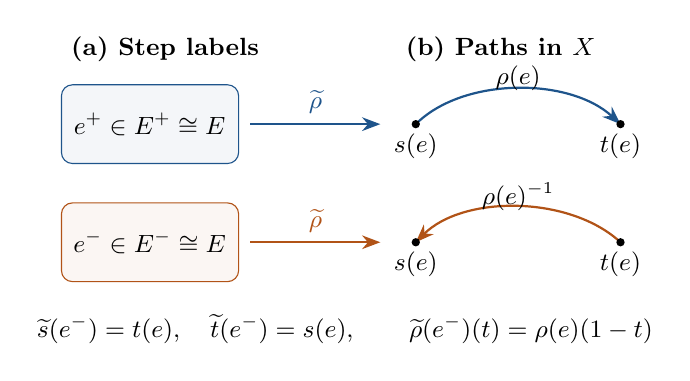
\begin{tikzpicture}[font=\small,>=Stealth]
\node[anchor=west,font=\small\bfseries] at (0,2.4) {(a) Step labels};
\draw[rounded corners,fill=pathblue!5,draw=pathblue] (0,0.95) rectangle (2.25,1.95);
\draw[rounded corners,fill=pathorange!5,draw=pathorange] (0,-0.55) rectangle (2.25,0.45);
\node at (1.12,1.45) {$e^+\in E^+\cong E$};
\node at (1.12,-0.05) {$e^-\in E^-\cong E$};
\draw[->,pathblue,thick] (2.4,1.45) -- node[above] {$\widetilde\rho$} (4.05,1.45);
\draw[->,pathorange,thick] (2.4,-0.05) -- node[above] {$\widetilde\rho$} (4.05,-0.05);
\node[anchor=west,font=\small\bfseries] at (4.25,2.4) {(b) Paths in $X$};
\draw[->,pathblue,thick] (4.5,1.45) .. controls (5.1,2.05) and (6.45,2.05) .. (7.1,1.45);
\fill (4.5,1.45) circle (1.5pt) node[below] {$s(e)$};
\fill (7.1,1.45) circle (1.5pt) node[below] {$t(e)$};
\node at (5.8,2.03) {$\rho(e)$};
\draw[<-,pathorange,thick] (4.5,-0.05) .. controls (5.1,0.55) and (6.45,0.55) .. (7.1,-0.05);
\fill (4.5,-0.05) circle (1.5pt) node[below] {$s(e)$};
\fill (7.1,-0.05) circle (1.5pt) node[below] {$t(e)$};
\node at (5.8,0.53) {$\rho(e)^{-1}$};
\node[align=center] at (3.6,-1.15) {$\widetilde s(e^-)=t(e),\quad
 \widetilde t(e^-)=s(e),\qquad
 \widetilde\rho(e^-)(t)=\rho(e)(1-t)$};
\end{tikzpicture}
\caption{Formal reversal changes the direction of a represented path and
leaves the topology of the step space unchanged.  The two curves depict the same geometric
route traversed in opposite directions.  Endpoint maps take values in $X$;
the realization map takes values in $X^I$.}
\label{fig:oriented-steps}
\end{figure}


For composable interval paths $\alpha$ and $\beta$ and $m,n\in\N$, write
$\alpha\star_{m,n}\beta$ for the length-weighted concatenation.  When
$m,n>0$, it is given by
\[
 (\alpha\star_{m,n}\beta)(t)=
 \begin{cases}
   \alpha\!\left(\dfrac{m+n}{m}t\right),
     &0\leq t\leq\dfrac{m}{m+n},\\[7pt]
   \beta\!\left(\dfrac{(m+n)t-m}{n}\right),
     &\dfrac{m}{m+n}\leq t\leq 1.
 \end{cases}
\]
Use the natural zero-length conventions
$\alpha\star_{0,n}\beta=\beta$ and
$\alpha\star_{m,0}\beta=\alpha$; when $m=n=0$, use the constant path at
the common endpoint.  Thus the two input paths occupy $m$ and $n$ equal
word slots, respectively.  For composable paths $\alpha$, $\beta$, and
$\gamma$ occupying $m$, $n$, and $k$ word slots, respectively, this gives the
following literal identities, including the zero-length cases under the stated
conventions:
\[
 (\alpha\star_{m,n}\beta)\star_{m+n,k}\gamma
 =\alpha\star_{m,n+k}(\beta\star_{n,k}\gamma),
 \qquad
 (\alpha\star_{m,n}\beta)^{-1}
 =\beta^{-1}\star_{n,m}\alpha^{-1}.
\]

\begin{example}[Reading the weights]
Suppose that $\alpha$ occupies two word slots and $\beta$ occupies one.
Then $\alpha\star_{2,1}\beta$ follows $\alpha$ until time $2/3$ and
follows $\beta$ on the remaining third of the interval.  If $\gamma$ also
occupies one slot, strict reassociation is visible in the concrete identity
\[
  (\alpha\star_{2,1}\beta)\star_{3,1}\gamma
  =\alpha\star_{2,2}(\beta\star_{1,1}\gamma).
\]
The weights record word-slot lengths and nothing else: no choice of
parenthesization and no geometric homotopy witness is involved.
\end{example}

\begin{definition}[geometric trace]
For $n\geq 1$, let $W_n\subseteq\widetilde E^n$ be the subspace of composable
words $(e_1,\ldots,e_n)$ satisfying
\(\widetilde t(e_i)=\widetilde s(e_{i+1})\) for every $i$.  Put $W_0=X$, representing empty traces,
with both endpoint maps equal to the identity on $X$, and define the
topological trace carrier by the disjoint union
\[
  \mathsf{Tr}_{\mathcal P}=\coprod_{n\in\N}W_n.
\]
Give $\N$ the discrete topology.  The length map is the coproduct index and
is continuous.  For $p=(e_1,\ldots,e_n)\in W_n$ with
$n\geq1$, define its realization by equal word slots,
\[
 |p|(t)=\widetilde\rho(e_i)(nt-i+1)
 \quad\text{for }1\leq i\leq n,\quad
 \frac{i-1}{n}\leq t\leq\frac{i}{n}.
\]
For $p\in W_0=X$, let $|p|$ be the constant path at its point.  We write
\(\Trace(a,b)\) for the set of words with endpoints $a,b$.  Empty words, word
concatenation, and reversal are the identity, composition, and inverse
operations on traces.  In particular, for $p\in W_m$ and
$q\in W_n$,
\[
 |p;q|=|p|\star_{m,n}|q|.
\]
Representing traces as flat words makes the unit, associativity,
double-inverse, and reversal-of-composite laws literal equalities.
Their equal-slot realizations satisfy the same equalities.
Inverse cancellation is different: a word followed by its reversal need
not be the empty word, and its realization contracts by a homotopy.

\end{definition}

\begin{lemma}[continuity of trace realization]
\label{lem:trace-realization-continuous}
The equal-slot realization map
\[
  |\cdot|:\mathsf{Tr}_{\mathcal P}\longrightarrow X^I
\]
is continuous for the coproduct trace topology.
\end{lemma}

\begin{proof}
On the zero-letter component $W_0=X$, the realization is the constant-path
map.  Its adjoint $X\times I\to X$, $(a,t)\mapsto a$, is continuous, so the
compact-open exponential law gives continuity into $X^I$.  Fix $n\geq1$.
For each $1\leq i\leq n$, the closed slot
\[
  C_i=W_n\times[(i-1)/n,i/n]\subseteq W_n\times I
\]
supports the continuous formula
\[
  (p,t)\longmapsto
  \widetilde\rho(e_i(p))(nt-i+1),
\]
where $e_i:W_n\to\widetilde E$ is the $i$th coordinate.  Continuity follows
from the continuity of $\widetilde\rho$ and of evaluation for the compact-open
topology.  On a
common boundary $t=i/n$, the two formulas agree because composability gives
\(\widetilde t(e_i)=\widetilde s(e_{i+1})\).  The pasting lemma therefore gives a continuous adjoint
\(W_n\times I\to X\).  Since $I$ is compact Hausdorff, the compact-open
exponential law gives a continuous map $W_n\to X^I$.  The coproduct
universal property now assembles these component maps into the displayed
realization map.
\end{proof}

The compact-open topology also gives continuous constant-path and reversal
maps on $X^I$.  On each fixed pair of length components, the weighted
operation $\star_{m,n}$ is continuous on the corresponding endpoint
pullback; the length coordinates are discrete, so these operations assemble
continuously over the coproduct.  Word concatenation and reversal are
continuous on the corresponding endpoint pullbacks of the $W_n$.  Together
with Lemma~\ref{lem:trace-realization-continuous}, these are the continuity
facts used below.  Nothing is assumed about products of quotient maps.

Let
\[
  \mathsf{Coh}_{\mathcal P}(p,\gamma)\;:\Longleftrightarrow\;
  \text{there exists an endpoint-fixed homotopy from $\gamma$ to $|p|$}.
\]
Only the existence of such a homotopy is required; the homotopy itself is
not an entry of the pair.  The coherent carrier is the set
\[
  T=\{(p,\gamma)\in\mathsf{Tr}_{\mathcal P}\times X^I:
      \gamma(0)=s(p),\ \gamma(1)=t(p),\ \mathsf{Coh}_{\mathcal P}(p,\gamma)\}.
\]
The two entries have different jobs.  The trace $p$ retains the finite
sequence of primitive steps to which the scoped rewrite relation applies,
while $\gamma$ is an independently chosen geometric representative observed
by the topology.  The coherence condition connects them without turning every
ambient homotopy into a syntactic rewrite.  The scoped quotient identifies all
coherent representatives of the same scoped trace class.  Thus $\gamma$
affects the representative topologies and defines the raw realization map,
but no particular choice of $\gamma$ survives in a quotient arrow.

\subsection*{Geometric meaning of coherence}
Having the same endpoints is necessary but not sufficient for coherence.
Let $A=(-1,0)$, $B=(0,1)$, and $C=(1,0)$ in $\mathbb R^2$.
Let $\alpha$ traverse the two straight segments $AB$ and $BC$ at equal
speed on the two halves of $I$, and put $\beta(t)=(2t-1,0)$.
In the plane,
\[
 H(u,t)=(1-u)\alpha(t)+u\beta(t)
\]
is a continuous homotopy from $\alpha$ to $\beta$ fixing $A,C$.
Thus, if $|p|=\alpha$, the pair $(p,\beta)$ is coherent.
If instead $X=\mathbb R^2\setminus\{(0,\tfrac13)\}$, both paths still
exist, but the loop $\alpha\star_{1,1}\beta^{-1}$ surrounds the missing
point once.  Its winding is nonzero, so no endpoint-fixed homotopy exists
in $X$ \cite{Hatcher02}.  Figure~\ref{fig:coherence} depicts this change.
Both paths remain continuous; what fails is that the loop between them cannot
be filled inside the specified space.

More generally, for parallel paths $\alpha,\beta$,
\[
 \alpha\simeq_{\partial I}\beta
 \quad\Longleftrightarrow\quad
 \alpha\star_{1,1}\beta^{-1}\simeq_{\partial I}c_{\alpha(0)}.
\]
This follows from the groupoid laws of endpoint-fixed homotopy classes.
A homotopy may be regarded as a path in $X^I(A,C)$, but the computational
trace remains a finite word.  A simple or discrete step space $E$ does not
remove obstructions in $X$ either.  Every named rewrite still needs a semantic
homotopy, and the existence of a homotopy does not by itself declare a scoped
rewrite.
\begin{figure}[htbp]
\centering
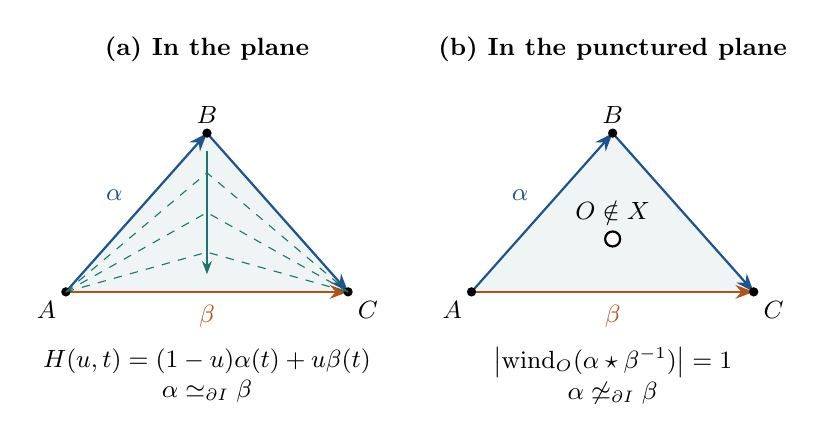
\begin{tikzpicture}[font=\small,>=Stealth,scale=1.12]
\foreach \x/\lab in {0/{(a) In the plane},4.6/{(b) In the punctured plane}} {
 \begin{scope}[xshift=\x cm]
 \node[font=\small\bfseries] at (1.6,2.75) {\lab};
 \fill[pathteal!7] (0,0) -- (1.6,1.8) -- (3.2,0) -- cycle;
 \draw[->,pathblue,thick] (0,0) -- (1.6,1.8);
 \draw[->,pathblue,thick] (1.6,1.8) -- (3.2,0);
 \draw[->,pathorange,thick] (0,0) -- (3.2,0);
 \fill (0,0) circle(1.5pt) node[below left] {$A$};
 \fill (1.6,1.8) circle(1.5pt) node[above] {$B$};
 \fill (3.2,0) circle(1.5pt) node[below right] {$C$};
 \node[pathblue] at (0.55,1.1) {$\alpha$};
 \node[pathorange] at (1.6,-0.28) {$\beta$};
 \end{scope}
}
\foreach \h in {0.45,0.9,1.35} {
 \draw[pathteal,dashed] (0,0) -- (1.6,\h) -- (3.2,0);
}
\draw[->,pathteal] (1.6,1.6) -- (1.6,0.2);
\draw[fill=white,thick] (6.2,0.6) circle(0.085);
\node[anchor=south,inner sep=1pt] at (6.2,0.77) {$O\notin X$};
\node[align=center] at (1.6,-0.95) {$H(u,t)=(1-u)\alpha(t)+u\beta(t)$\\
 $\alpha\simeq_{\partial I}\beta$};
\node[align=center] at (6.2,-0.95) {$\left|\operatorname{wind}_{O}
 (\alpha\star\beta^{-1})\right|=1$\\
 $\alpha\not\simeq_{\partial I}\beta$};
\end{tikzpicture}
\caption{Coherence requires a homotopy inside the chosen ambient space.
Left: intermediate broken paths move $B$ to the segment $AC$, keeping $A,C$
fixed.  Right: deleting the interior point $O=(0,\tfrac13)$ prevents any
such homotopy, although both boundary paths remain continuous.
For $|p|=\alpha$, $(p,\beta)$ is coherent only in the left-hand example.
The shaded triangle is available in (a), but is not a filling in (b).}
\label{fig:coherence}
\end{figure}


We now put two canonical topologies on this same coherent carrier.  First,
let
\[
  \kappa_{\mathrm{tr}}:T\longrightarrow
    \mathsf{Tr}_{\mathcal P}\times X^I,
  \qquad
  \kappa_{\mathrm{tr}}(p,\gamma)=(p,\gamma).
\]
The \emph{trace-sensitive topology} $T_{\mathrm{tr}}$ is the initial topology
induced by $\kappa_{\mathrm{tr}}$; because $T$ is a subset of
$\mathsf{Tr}_{\mathcal P}\times X^I$, this is just the subspace topology.
In it, the complete finite word is a topological coordinate.  Second, let
\[
  \kappa_{\mathrm{obs}}:T\longrightarrow X\times X\times\N\times X^I\times X^I,
  \qquad
  \kappa_{\mathrm{obs}}(p,\gamma)=(s(p),t(p),\ell(p),|p|,\gamma).
\]
The \emph{observable topology} $T_{\mathrm{obs}}$ is the initial topology
induced by $\kappa_{\mathrm{obs}}$:
it is the coarsest topology making these semantic observables continuous.
Since the endpoint maps, length, and realization are continuous on the trace
carrier, $\kappa_{\mathrm{obs}}$ factors continuously through
$\kappa_{\mathrm{tr}}$.  Consequently the identity
\[
  i_T:T_{\mathrm{tr}}\longrightarrow T_{\mathrm{obs}}
\]
is continuous; that is, the trace-sensitive topology is finer than the
observable one.

Unless a superscript says otherwise, Sections~\ref{sec:quotient}--\ref{sec:circle-torus} use $T_{\mathrm{obs}}$ and
its quotient, and we write $T:=T_{\mathrm{obs}}$ and
$T^{(2)}:=T_{\mathrm{obs}}^{(2)}$.  The results of Sections~\ref{sec:quotient}, \ref{sec:functoriality}, \ref{sec:comparison}, and~\ref{sec:universal}
hold verbatim for $T_{\mathrm{tr}}$.  Their proofs use continuity of raw maps
on the carrier, which Lemma~\ref{lem:coherent-operations-continuous} and the
coordinate arguments of Sections~\ref{sec:functoriality} and~\ref{sec:universal} give for both topologies, and
quotient criteria that do not care which topology the carrier has.  Geometric
completeness is a property of equivalence relations, so it does not depend on
the choice at all.  Section~\ref{sec:final-ordinary} is the exception, since compatibility of the
final and ordinary topologies has to be checked for each representative
topology separately.  Proposition~\ref{prop:trace-sensitive-refinement}
compares the two resulting quotients.

For the observable choice, write $\kappa=\kappa_{\mathrm{obs}}$.
Its five coordinates record the source, target, word length, realized trace,
and chosen geometric path.  They determine the topology, but not the
equivalence relation used in the scoped quotient.  Two distinct traces can
have the same five coordinates without being related by the allowed rewrites.

For $*=\mathrm{tr},\mathrm{obs}$, define the common composable set with its
chosen subspace topology by
\[
  T_*^{(2)}=\{(u,v)\in T_*\times T_*:t(u)=s(v)\}.
\]

\begin{proposition}[trace-sensitive refinement]
\label{prop:trace-sensitive-refinement}
Let $T_{\mathrm{tr}}$ and $T_{\mathrm{obs}}$ denote the two topologies above.
The identity $i_T:T_{\mathrm{tr}}\to T_{\mathrm{obs}}$ is continuous, and its
restriction to the common composable set is continuous:
\[
  i_T^{(2)}:T_{\mathrm{tr}}^{(2)}\longrightarrow T_{\mathrm{obs}}^{(2)}.
\]
Let $G_{\mathcal P}^{\mathrm{tr}}$ and $G_{\mathcal P}^{\mathrm{obs}}$ be
the quotient arrow spaces for the same scoped relation, formed from the two
representative topologies.  Then the identity on quotient sets induces a
continuous bijection
\[
  J:G_{\mathcal P}^{\mathrm{tr}}\longrightarrow G_{\mathcal P}^{\mathrm{obs}},
  \qquad J\,q_{\mathrm{tr}}=q_{\mathrm{obs}}\,i_T.
\]
The corresponding map on final composable-pair quotients is continuous as
well.  In general $J^{-1}$ need not be continuous, so $J$ need not be a
homeomorphism (Example~\ref{ex:quotient-topology-separation}).
\end{proposition}

\begin{proof}
The factorization of $\kappa_{\mathrm{obs}}$ through $\kappa_{\mathrm{tr}}$
proves continuity of $i_T$ by the initial-topology criterion.  Restriction to
the endpoint pullback gives $i_T^{(2)}$.  The identity preserves the scoped
equivalence relation, so it descends to $J$.  Since
$q_{\mathrm{tr}}$ is a quotient map and
$J\,q_{\mathrm{tr}}=q_{\mathrm{obs}}\,i_T$ is continuous, the quotient
criterion proves continuity of $J$.  The same argument applies to the
componentwise final composable-pair quotients.
\end{proof}

\begin{proposition}[when trace sensitivity disappears]
\label{prop:trace-collapse-section}
Let $P_{\mathcal P}\subseteq X^I$ be the space of paths represented by
coherent pairs, with its subspace topology.  Write
$\pi_{\mathrm{obs}}:T_{\mathrm{obs}}\to P_{\mathcal P}$ and
$\pi_{\mathrm{tr}}:T_{\mathrm{tr}}\to P_{\mathcal P}$ for the maps that
forget the trace.  Suppose that $\mathcal P$ is geometrically complete and
that $\pi_{\mathrm{tr}}$ has a continuous section
$s:P_{\mathcal P}\to T_{\mathrm{tr}}$.  Then the quotient comparison
$J:G_{\mathcal P}^{\mathrm{tr}}\to G_{\mathcal P}^{\mathrm{obs}}$ is a
homeomorphism.
\end{proposition}

\begin{proof}
The observable code makes $\pi_{\mathrm{obs}}$ continuous.  Thus
$\theta=s\pi_{\mathrm{obs}}:T_{\mathrm{obs}}\to T_{\mathrm{tr}}$ is
continuous.  For each coherent pair $u$, the chosen paths of $u$ and
$\theta(u)$ are equal.  Geometric completeness makes their scoped classes
equal, so $q_{\mathrm{tr}}\theta=J^{-1}q_{\mathrm{obs}}$.  Since
$q_{\mathrm{obs}}$ is quotient, $J^{-1}$ is continuous.  The forward map
is continuous by Proposition~\ref{prop:trace-sensitive-refinement}.
\end{proof}

The hypothesis is a continuous choice of trace for each represented path;
completeness alone is not used to choose one.  The universal one-letter
section supplies such a choice.  On the circle and torus based-loop
presentations, a standard word selected by winding also gives a section:
winding is locally constant in the compact-open based-loop space, and the
geometric-path coordinate varies continuously.  Thus the two quotient
topologies agree on those based-loop examples.

\begin{example}[Same geometry, different computation]
Suppose $p,q\in W_n$ have the same endpoints and the same equal-slot
realization, and let $\gamma$ be a common coherent representative.  If
$p\neq q$, then $(p,\gamma)$ and $(q,\gamma)$ have identical observable
codes.  They are therefore topologically indistinguishable in
$T_{\mathrm{obs}}$, even though the scoped quotient identifies them only when
$p\RwEq q$.  If the trace carrier is Hausdorff, the trace-sensitive topology
$T_{\mathrm{tr}}$ can separate these two computationally different points.
The allowed rewrites are the same in both cases; only the power of the
topology to distinguish points changes.
\end{example}

\begin{example}[A separation that survives the quotient]
\label{ex:quotient-topology-separation}
Let $X=\mathbb R/\mathbb Z$ and let $E=\{e,f\}$ be discrete.
Both steps are based at $0$ and realize the same nonconstant loop
$\lambda(t)=[t]$.  Declare no named rewrites; the scoped relation contains
only the structural groupoid laws.  Write
\[
  u_e=(e,\lambda),\qquad u_f=(f,\lambda),
\]
for two coherent points.  Assign signed count $(1,0)$ to $e$ and $(0,1)$
to $f$, extend by addition over concatenation, and negate under reversal.
This map from traces to $\mathbb Z^2$ respects every structural groupoid
law.  It separates the scoped classes of $u_e$ and $u_f$, despite their
identical realized loops.  Because the trace space retains the full word
and $E$ is discrete, the signed-count map is continuous to discrete
$\mathbb Z^2$.  It descends to a continuous map on
$G_{\mathcal P}^{\mathrm{tr}}$, whose inverse image of $\{(1,0)\}$ is open,
contains $q_{\mathrm{tr}}(u_e)$, and excludes $q_{\mathrm{tr}}(u_f)$.

The observable codes of $u_e$ and $u_f$ are identical: both have the same
endpoints, length, realization, and coherent representative.  They are
therefore topologically indistinguishable in $T_{\mathrm{obs}}$.  An open
subset of $G_{\mathcal P}^{\mathrm{obs}}$ containing $q_{\mathrm{obs}}(u_e)$
would pull back to an observable-open set containing $u_e$, hence also $u_f$.
Thus it must contain $q_{\mathrm{obs}}(u_f)$.  The continuous bijection
$J:G_{\mathcal P}^{\mathrm{tr}}\to G_{\mathcal P}^{\mathrm{obs}}$ from
Proposition~\ref{prop:trace-sensitive-refinement} is therefore not a
homeomorphism.  The difference comes from two labels for one nonconstant loop.
Figure~\ref{fig:same-geometry} summarizes the separation mechanism.
\end{example}

\begin{figure}[htbp]
\centering
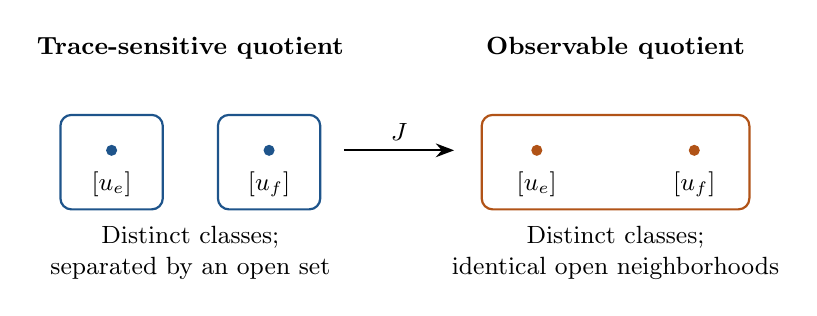
\begin{tikzpicture}[font=\small,>=Stealth]
\node[font=\small\bfseries] at (0,1.6) {Trace-sensitive quotient};
\node[font=\small\bfseries] at (5.4,1.6) {Observable quotient};
\draw[pathblue,thick,rounded corners] (-1.65,-0.45) rectangle (-0.35,0.75);
\draw[pathblue,thick,rounded corners] (0.35,-0.45) rectangle (1.65,0.75);
\fill[pathblue] (-1,0.3) circle (2pt);
\fill[pathblue] (1,0.3) circle (2pt);
\node[below] at (-1,0.15) {$[u_e]$};
\node[below] at (1,0.15) {$[u_f]$};
\draw[pathorange,thick,rounded corners] (3.7,-0.45) rectangle (7.1,0.75);
\fill[pathorange] (4.4,0.3) circle (2pt);
\fill[pathorange] (6.4,0.3) circle (2pt);
\node[below] at (4.4,0.15) {$[u_e]$};
\node[below] at (6.4,0.15) {$[u_f]$};
\draw[->,thick] (1.95,0.3) -- (3.35,0.3) node[midway,above] {$J$};
\node[align=center] at (0,-1) {Distinct classes;\\separated by an open set};
\node[align=center] at (5.4,-1) {Distinct classes;\\identical open neighborhoods};
\end{tikzpicture}
\caption{The two quotients identify the same arrows and differ only in
their topology.
In Example~\ref{ex:quotient-topology-separation}, both steps realize the
same nonconstant circle loop, but their signed-count values differ. The map $J$
preserves both scoped classes.  In the observable quotient every open set
containing either class contains both.  Boxes illustrate separation properties
only; the shared box is not asserted to be an open two-point subset.}
\label{fig:same-geometry}
\end{figure}


\begin{example}[One trace, two coherent representatives]
Let $p$ be a trace and let $\gamma$ and $\delta$ be endpoint-fixed homotopic
representatives with
\[
  \gamma\simeq_{\partial I}|p|\simeq_{\partial I}\delta.
\]
Then $(p,\gamma)$ and $(p,\delta)$ are both points of $T$.  The observable
topology may observe the difference between their fifth coordinates, but the
scoped quotient identifies them because the trace coordinate is the same.
A coherent representative is therefore useful before quotienting without
becoming extra data in a quotient arrow.
\end{example}

For $u=(p,\gamma)\in T$, put $s(u)=s(p)$ and $t(u)=t(p)$.

\begin{lemma}[continuity of coherent operations]\label{lem:coherent-operations-continuous}
For either $*=\mathrm{tr}$ or $*=\mathrm{obs}$, let $\iota:X\to T_*$ send
$a$ to the coherent identity $(1_a,c_a)$, let $\sigma:T_*\to T_*$ send
$(p,\gamma)$ to
$(p^{-1},\gamma^{-1})$, and let
\[
  \mu_*:T_*^{(2)}\longrightarrow T_*,
  \qquad ((p,\gamma),(q,\delta))\longmapsto
    (p;q,\gamma\star_{\ell(p),\ell(q)}\delta),
\]
where the weighted operation uses the discrete trace lengths.  Then all three
maps are continuous.
\end{lemma}

\begin{proof}
For $T_{\mathrm{obs}}$, it is enough to check continuity after applying
$\kappa_{\mathrm{obs}}$.  The three resulting observable codes are respectively
\[
  (a,a,0,c_a,c_a),
\quad
  (t(p),s(p),\ell(p),|p|^{-1},\gamma^{-1}),
\]
and, on the composable pullback,
\[
  \bigl(s(p),t(q),\ell(p)+\ell(q),
    |p|\star_{\ell(p),\ell(q)}|q|,
    \gamma\star_{\ell(p),\ell(q)}\delta\bigr).
\]
The first is continuous because constant paths depend continuously on $a$;
the second uses reversal on $X^I$; and the third uses addition on the discrete
length coordinate and continuity of the weighted operation on each fixed
length component.  Each code depends continuously only on the observable
codes of the input(s), so the initial-topology criterion proves continuity of
all three operations.  For $T_{\mathrm{tr}}$, the corresponding first
coordinates are the continuous word maps
$a\mapsto 1_a$, $p\mapsto p^{-1}$, and $(p,q)\mapsto p;q$ on the trace
carrier; the second coordinates are the same continuous path operations just
used.  The initial-topology criterion for $\kappa_{\mathrm{tr}}$ therefore
proves continuity in the trace-sensitive topology as well.  Reversal and
weighted concatenation preserve the coherence predicate by reversing and
concatenating the endpoint-fixed homotopies.  The Lean development flattens
the parenthesized internal trace to a signed word so that these
first-coordinate maps can be checked.
\end{proof}

\begin{definition}[scoped presentation]
A continuous geometric rewrite presentation $\mathcal P$ on $(X,E)$ consists
of a predicate
\[
  \mathsf{Rule}_{\mathcal P}(p,q),\qquad p,q:\Trace(a,b),
\]
and, for every instance of $\mathsf{Rule}_{\mathcal P}(p,q)$, an endpoint-fixed homotopy
between the realizations of $p$ and $q$.
\end{definition}

Here $\mathsf{Rule}_{\mathcal P}$ specifies the named rewrites; it should
not be confused with the realization comparison $R_{\mathcal P}$ of Section~\ref{sec:comparison}.
The definition asks for a homotopy witness for each named rewrite and imposes
no completeness condition.

\begin{definition}[scoped rewrite equality]\label{def:scoped-rewrite-equality}
For parallel traces, write $p\RwEq q$ for the inductively generated relation
whose constructors are reflexivity, the named generators $\mathsf{Rule}_{\mathcal P}$,
symmetry, transitivity, congruence under concatenation and reversal, and the
following structural groupoid coherences:
\[
\begin{array}{lll}
(1_a);p\RwEq p, & p;(1_b)\RwEq p, & (p;q);r\RwEq p;(q;r),\\
p^{-1};p\RwEq 1_b, & p;p^{-1}\RwEq 1_a, & (p^{-1})^{-1}\RwEq p,\\
(1_a)^{-1}\RwEq 1_a, & (p;q)^{-1}\RwEq q^{-1};p^{-1}. &
\end{array}
\]
Only the rules declared by $\mathcal P$ and these structural constructors are
available.  Literal equality of traces is handled by reflexivity and
substitution; ambient homotopy of their realizations is not an additional
constructor.
\end{definition}

\begin{lemma}[weighted concatenation invariance]
\label{lem:weighted-concat-invariance}
Let $\alpha\simeq_{\partial I}\alpha'$ and
$\beta\simeq_{\partial I}\beta'$ be endpoint-fixed homotopies of composable
paths.  Write $c_x$ for the constant path at $x$, and assume explicitly that
\[
\begin{aligned}
m=0&\Rightarrow \alpha(0)=\alpha(1)\ \text{and}\ \alpha\simeq_{\partial I}c_{\alpha(0)},\\
n=0&\Rightarrow \beta(0)=\beta(1)\ \text{and}\ \beta\simeq_{\partial I}c_{\beta(0)},\\
m'=0&\Rightarrow \alpha'(0)=\alpha'(1)\ \text{and}\ \alpha'\simeq_{\partial I}c_{\alpha'(0)},\\
n'=0&\Rightarrow \beta'(0)=\beta'(1)\ \text{and}\ \beta'\simeq_{\partial I}c_{\beta'(0)}.
\end{aligned}
\]
For arbitrary
$m,n,m',n'\in\N$, with the zero-length conventions above,
\[
  \alpha\star_{m,n}\beta
  \simeq_{\partial I}
  \alpha'\star_{m',n'}\beta'.
\]
\end{lemma}

\begin{proof}
When all four weights are positive, let $\lambda_{m,n}:[0,1]\to[0,1]$ be
the piecewise-linear endpoint-fixing homeomorphism that maps
$m/(m+n)$ to $1/2$ and is linear on the two sides.  Explicitly,
\[
 \lambda_{m,n}(t)=
 \begin{cases}
   \dfrac{m+n}{2m}t,
     &0\leq t\leq\dfrac{m}{m+n},\\[6pt]
   \dfrac12+\dfrac{m+n}{2n}\left(t-\dfrac{m}{m+n}\right),
     &\dfrac{m}{m+n}\leq t\leq1.
 \end{cases}
\]
Then
\[
  \alpha\star_{m,n}\beta
  =(\alpha\star_{1,1}\beta)\circ\lambda_{m,n}.
\]
The straight-line homotopy $(1-u)\lambda_{m,n}+u\lambda_{m',n'}$ fixes $0$ and
$1$, so changing the breakpoint gives an endpoint-fixed reparametrization
homotopy.  Horizontal concatenation of the
given homotopies at the common breakpoint $1/2$ gives
\[
  \alpha\star_{1,1}\beta
  \simeq_{\partial I}
  \alpha'\star_{1,1}\beta'.
\]
Combining these homotopies proves the claim when all weights are positive.
If a weight is zero, first use the corresponding zero-slot hypothesis to replace
the corresponding factor by the constant path at its endpoint.  Such a factor
has coinciding endpoints by the displayed hypothesis, so the stated
convention then deletes that constant factor.  When the zero/nonzero status
changes between the two sides, this replacement inserts or removes the factor
up to endpoint-fixed homotopy.  The remaining positive-weight factors are
handled by the preceding reparametrization argument; when both weights are
zero, the convention yields the common endpoint constant.  Thus all
zero-length cases follow as well.
\end{proof}

\begin{theorem}[realization soundness]
\label{thm:realization-soundness}
If $p\RwEq q$, then the realized paths are endpoint-fixed homotopic.
\end{theorem}

\begin{proof}
Induct on the derivation of $p\RwEq q$.  Reflexivity is the constant
homotopy, and a named generator is sound by the corresponding presentation
witness.  Symmetry and transitivity use symmetry and vertical composition of
endpoint-fixed homotopies.  In the concatenation-congruence case, apply the
weighted concatenation invariance lemma to the two inductive homotopies and
the four trace lengths; this accounts for rewrites that change word length.
The zero-weight hypotheses of that lemma hold because a trace of length zero
is an empty word, whose realization is a constant path.
For reversal, reverse the path parameter, replacing a homotopy $H(s,t)$ by
$H(s,1-t)$.  Unit, associativity,
double-reversal, and reversal of a composite are literal equalities for the
flat word realization, hence use reflexive homotopies.  The two
inverse-cancellation cases use the standard
endpoint-fixed contraction homotopies made explicit below.  This covers every rule that can occur in a scoped derivation.
\end{proof}

\begin{lemma}[backtracking contracts in every space]
\label{lem:backtracking}
For any continuous path $\alpha:I\to X$, the formula
\[
 H(u,t)=\alpha\!\left(\min\{2t,\,2(1-t),\,1-u\}\right)
 \qquad (u,t\in I)
\]
is an endpoint-fixed homotopy from
$\alpha\star_{1,1}\alpha^{-1}$ to $c_{\alpha(0)}$.
\end{lemma}
\begin{proof}
The minimum is a continuous map $I^2\to I$, so $H$ is continuous.
At $u=0$ its argument is the triangular function
$\min\{2t,2(1-t)\}$, which traverses $\alpha$ and then retraces it.
At $u=1$ it is identically zero, and for every $u$ its values at
$t=0,1$ are zero.  These are the required boundary conditions.
Applying the same construction to $\alpha^{-1}$ proves the other inverse law.
\end{proof}

The homotopy stays entirely in $\alpha(I)$: no disk in $X$ is needed.
For a nonempty trace $p$, the two factors in $p;p^{-1}$ have equal length,
so its weighted realization is exactly the half-interval concatenation
in Lemma~\ref{lem:backtracking}; the empty case is constant.
Figure~\ref{fig:backtracking} makes the contrast with
Figure~\ref{fig:coherence} explicit.
\begin{figure}[htbp]
\centering
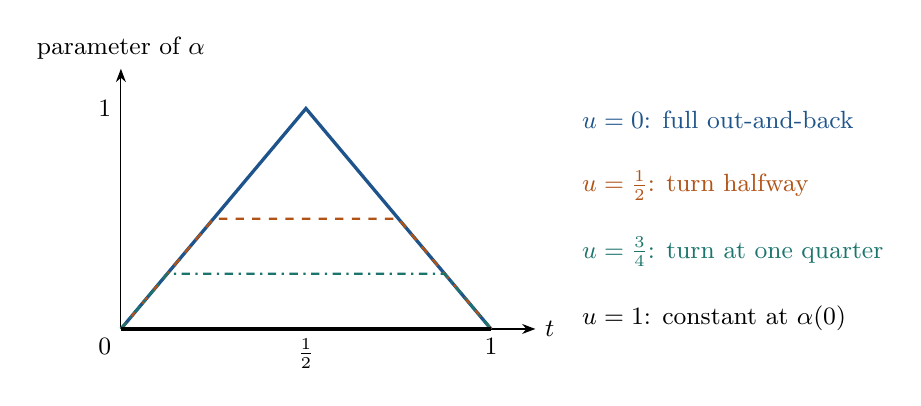
\begin{tikzpicture}[font=\small,>=Stealth,x=4.7cm,y=2.8cm]
\draw[->] (0,0) -- (1.12,0) node[right] {$t$};
\draw[->] (0,0) -- (0,1.18) node[above] {parameter of $\alpha$};
\draw[pathblue,very thick] (0,0) -- (0.5,1) -- (1,0);
\draw[pathorange,thick,dashed] (0,0) -- (0.25,0.5) -- (0.75,0.5) -- (1,0);
\draw[pathteal,thick,dash dot] (0,0) -- (0.125,0.25) -- (0.875,0.25) -- (1,0);
\draw[black,very thick] (0,0) -- (1,0);
\node[below left] at (0,0) {$0$};
\node[below] at (0.5,0) {$\tfrac12$};
\node[below] at (1,0) {$1$};
\node[left] at (0,1) {$1$};
\node[pathblue,anchor=west] at (1.22,0.95) {$u=0$: full out-and-back};
\node[pathorange,anchor=west] at (1.22,0.65) {$u=\tfrac12$: turn halfway};
\node[pathteal,anchor=west] at (1.22,0.35) {$u=\tfrac34$: turn at one quarter};
\node[anchor=west] at (1.22,0.05) {$u=1$: constant at $\alpha(0)$};
\end{tikzpicture}
\caption{Backtracking cancellation as an explicit homotopy.
The plotted function is $r_u(t)=\min\{2t,2(1-t),1-u\}$;
the actual path is $H(u,t)=\alpha(r_u(t))$.
As $u$ increases, the turning point retreats along $\alpha$ and the path
waits there before returning.  All intermediate paths stay in $\alpha(I)$,
so even a hole surrounded by $\alpha$ cannot obstruct this cancellation.}
\label{fig:backtracking}
\end{figure}


\begin{remark}
The soundness theorem is one-way.  Equality of realized geometric homotopy
classes does not imply scoped rewrite equality unless a separate geometric
completeness theorem is proved.  Because the implication runs in only one
direction, the presentation can retain computational information.
\end{remark}

\section{The quotient groupoid and its universal property}
\label{sec:quotient}

For coherent traces $u=(p,\gamma)$ and $v=(q,\delta)$, write
$u\approx v$ when their endpoints agree and $p\RwEq q$.  By realization
soundness, equivalent coherent traces determine the same endpoint-fixed
homotopy class of geometric paths.  The quotient arrow space is
\[
  G_{\mathcal P}=T/{\approx},
\]
with the quotient topology induced by $q:T\to G_{\mathcal P}$.  Endpoint
maps descend to continuous maps
\[
  s,t:G_{\mathcal P}\longrightarrow X.
\]
Reflexive paths and reversal descend because the scoped relation is closed
under the corresponding constructors.

The explicit composable carrier is the $T^{(2)}$ defined in Section~\ref{sec:traces}.
Its quotient relation is componentwise scoped equivalence, and its quotient is
denoted $G_{\mathcal P}^{(2),\Fin}$.  Write
\[
  q_{\Fin}^{(2)}:T^{(2)}\longrightarrow G_{\mathcal P}^{(2),\Fin}
\]
for the quotient map.  Concatenation of representatives gives a well-defined
map
\[
  m_{\Fin}:G_{\mathcal P}^{(2),\Fin}\longrightarrow G_{\mathcal P}.
\]
The composite $q\circ\mu:T^{(2)}\to G_{\mathcal P}$ is continuous and
constant on equivalent pairs.  The quotient criterion therefore makes
$m_{\Fin}$ continuous.  This argument uses the quotient of composable
representatives, not a product of quotient maps.

\begin{definition}[final-domain topological groupoid]
Let $G\rightrightarrows X$ be a groupoid with topologies on $G$ and $X$
such that source, target, identity, and inverse are continuous.
Give the set of composable arrow pairs $G\times_XG$ a topology, denoted
$C_{\mathrm{fin}}$, for which both projections $C_{\mathrm{fin}}\to G$ are
continuous.  We call these data a
\emph{final-domain topological groupoid} when multiplication
\[
  m:C_{\mathrm{fin}}\longrightarrow G
\]
is continuous.  The groupoid laws are the usual algebraic ones.  The topology
$C_{\mathrm{fin}}$ is part of the structure.  It is at least as fine as the
subspace topology from $G\times G$, and it may be strictly finer.
\end{definition}

Taken alone, the definition is weak: the discrete topology on
$C_{\mathrm{fin}}$ always qualifies.  What matters below is that
$G_{\mathcal P}$ comes with a canonical choice, the quotient topology from
explicitly composable representatives.  Section~\ref{sec:final-ordinary} compares that choice with
the subspace topology.

\begin{theorem}[canonical final-domain groupoid]
\label{thm:final-groupoid}
For every continuous geometric rewrite presentation $\mathcal P$:
\begin{enumerate}[label=(\alph*),leftmargin=2.2em]
\item $s,t$, the identity map $X\to G_{\mathcal P}$, and reversal
  $G_{\mathcal P}\to G_{\mathcal P}$ are continuous;
\item $m_{\Fin}$ and the two projections
  $G_{\mathcal P}^{(2),\Fin}\to G_{\mathcal P}$ are continuous;
\item the descended operations satisfy the left and right unit laws, inverse
  laws, and associativity.
\end{enumerate}
Thus $G_{\mathcal P}$ is a final-domain topological groupoid.
\end{theorem}

\begin{proof}
By Lemma~\ref{lem:coherent-operations-continuous}, the raw identity,
reversal, and concatenation maps are continuous for the stated topology.
Continuity of the endpoint maps and identities follows from the quotient
criterion, because the corresponding raw maps are continuous.  The same
argument applies to reversal.  The raw concatenation map
$T^{(2)}\to T$ is continuous and respects the componentwise quotient
relation, so it descends to $m_{\Fin}$; continuity follows from the defining
quotient topology on $G_{\mathcal P}^{(2),\Fin}$.  The $i$th projection
satisfies $\mathrm{pr}_i\circ q_{\Fin}^{(2)}=q\circ\mathrm{pr}_i$, so it is
continuous by the same criterion.

For the algebraic laws, choose representatives.  In the flat word model,
left and right units, associativity, double reversal, and reversal of a
composite are literal equalities of traces and of the weighted realizations;
their scoped witnesses are therefore reflexive structural coherences.  The
two inverse laws are not literal equalities.  They need endpoint-fixed
contraction homotopies and are represented by the constructors $p^{-1};p\RwEq 1_b$ and
$p;p^{-1}\RwEq 1_a$.  The quotient soundness criterion then turns each
scoped derivation into equality of quotient arrows.
The result is independent of representative choice because concatenation was
defined through the componentwise quotient.
\end{proof}



The next theorem describes which interpretations of coherent traces pass
through $G_{\mathcal P}$.  Such an interpretation must respect the rewrites
and the groupoid operations.  It must also give the same value to
$(p,\gamma)$ and $(p,\delta)$ whenever both are coherent: the scoped quotient
does not retain the choice of geometric representative.

\begin{theorem}[semantic factorization]\label{thm:semantic-factorization}
Let $\mathcal H\rightrightarrows X$ be a topological groupoid, and let
$\varphi:T\to\mathcal H_1$ be continuous.  Assume that $\varphi$ preserves
endpoints, identities, reversal, and concatenation, and that every named
rewrite of $\mathcal P$ is sent to an equality in $\mathcal H_1$ for every
choice of coherent representatives.  Assume moreover that $\varphi$ is
invariant under changing the coherent representative: whenever
$(p,\gamma),(p,\delta)\in T$, one has
\[
  \varphi(p,\gamma)=\varphi(p,\delta).
\]
Then there is a unique continuous map
\[
  \overline{\varphi}:G_{\mathcal P}\longrightarrow\mathcal H_1
\]
such that $\overline{\varphi}\,q=\varphi$.  The map
$\overline{\varphi}$ preserves all groupoid operations, with composition on
the source interpreted on $G_{\mathcal P}^{(2),\Fin}$.
\end{theorem}

\begin{proof}
Every trace $p$ has the coherent representative $(p,|p|)$, and representative
invariance gives $\varphi(p,\gamma)=\varphi(p,|p|)$ for every coherent
$(p,\gamma)$.  It therefore suffices to show that $p\RwEq q$ implies
$\varphi(p,|p|)=\varphi(q,|q|)$, by induction on the derivation.  Named
rewrites are covered by hypothesis, and reflexivity, symmetry, and
transitivity are immediate.  Since
$\mu((p,|p|),(q,|q|))=(p;q,|p;q|)$ and $\sigma(p,|p|)=(p^{-1},|p^{-1}|)$,
preservation of concatenation and reversal handles the two congruence cases.
The structural coherences hold because $\mathcal H$ satisfies the groupoid
laws and $\varphi$ preserves identities, reversal, and concatenation.  Hence
$\varphi$ is constant on $\approx$.  The quotient universal property gives a unique map
$\overline{\varphi}$, and the quotient criterion gives continuity.  The
operation-preservation equations hold on representatives and hence descend.
For composition, the same argument is applied to the quotient map
$T^{(2)}\to G_{\mathcal P}^{(2),\Fin}$; no product-quotient assumption is
needed.
\end{proof}

\section{Final and ordinary composable-pair topologies}
\label{sec:final-ordinary}

As before, $G_{\mathcal P}=G_{\mathcal P}^{\mathrm{obs}}$ and
$T=T_{\mathrm{obs}}$.  The definitions and theorems of this section apply
equally to the trace-sensitive quotient.  Compatibility for one
representative topology does not imply compatibility for the other, however;
the continuous map $J$ of Proposition~\ref{prop:trace-sensitive-refinement}
does not transfer it in either direction.

There is another natural composable domain.  Let
\[
  G_{\mathcal P}^{(2),\Ord}
  =\{(x,y)\in G_{\mathcal P}\times G_{\mathcal P}:t(x)=s(y)\}
\]
with the subspace topology.  The underlying set of this space is the same as
the underlying set of the final domain, but its topology need not be the same.
The canonical ordinary-pair map is
\[
  q_{\Ord}^{(2)}:T^{(2)}\longrightarrow G_{\mathcal P}^{(2),\Ord}.
\]
It is continuous and surjective.  There is a unique bijection
\[
  j:G_{\mathcal P}^{(2),\Fin}\longrightarrow G_{\mathcal P}^{(2),\Ord}
\]
such that
\[
  q_{\Ord}^{(2)}=j\circ q_{\Fin}^{(2)}.
\]
The map $j$ is continuous because $q_{\Fin}^{(2)}$ is quotient.  Products of
quotient maps need not be quotient maps, so $q_{\Ord}^{(2)}$ being quotient is
an extra property; it does not follow formally from $q$ being quotient.

\begin{definition}[product-quotient compatibility]
The presentation has product-quotient compatibility if $q_{\Ord}^{(2)}$ is a
quotient map onto the ordinary composable-pair space.  Since
$q_{\Ord}^{(2)}=j\circ q_{\Fin}^{(2)}$ and $q_{\Fin}^{(2)}$ is quotient, this
is equivalent to $j$ being a quotient map.
\end{definition}

The two domains have the same elements: composable pairs of scoped classes.
They differ only in their open sets.  For the final topology, a set $U$ is
open exactly when
\[
  \bigl(q_{\Fin}^{(2)}\bigr)^{-1}(U)
  \quad\text{is open in }T^{(2)}.
\]
For the ordinary topology, openness is inherited from
$G_{\mathcal P}\times G_{\mathcal P}$.
The final topology is always at least as fine as the ordinary one, since
$j$ is continuous.  Product-quotient compatibility says that there are no
additional open sets in the final topology.



\begin{theorem}[ordinary/final comparison]
\label{thm:ordinary-final}
For every presentation $\mathcal P$, the following are equivalent:
\begin{enumerate}[label=(\arabic*),leftmargin=2.2em]
\item $q_{\Ord}^{(2)}:T^{(2)}\to G_{\mathcal P}^{(2),\Ord}$ is a quotient map;
\item $j:G_{\mathcal P}^{(2),\Fin}\to G_{\mathcal P}^{(2),\Ord}$ is a
  quotient map;
\item the inverse bijection $j^{-1}:G_{\mathcal P}^{(2),\Ord}\to
  G_{\mathcal P}^{(2),\Fin}$ is continuous;
\item $j$ is a homeomorphism, equivalently the final and ordinary
  composable-pair topologies coincide.
\end{enumerate}
Thus each condition is also equivalent to product-quotient compatibility.
When these conditions hold, multiplication is continuous from the ordinary
pullback domain.  Theorem~\ref{thm:final-groupoid} uses none of these
conditions.
\end{theorem}

\begin{proof}
If $j$ is quotient, so is the composite $q_{\Ord}^{(2)}=j\circ q_{\Fin}^{(2)}$.
Conversely, suppose $q_{\Ord}^{(2)}$ is quotient and $j^{-1}(U)$ is open.  Then
$(q_{\Ord}^{(2)})^{-1}(U)=(q_{\Fin}^{(2)})^{-1}(j^{-1}(U))$ is open, so $U$ is
open.  This proves that (1) and (2) are equivalent.

The map $j$ is a continuous bijection.  A bijective quotient map has
continuous inverse, so (2) and (3) are equivalent; together with the already
known continuity of $j$, these are equivalent to (4).  The homeomorphism
condition is precisely equality of the two topologies on the common
underlying set.  Finally, when these conditions hold, multiplication is
continuous by the quotient criterion applied to its continuous
representative-level concatenation.
\end{proof}

\begin{remark}[terminology]
In the standard definition of a topological groupoid, multiplication is
continuous on the ordinary pullback $G_{\mathcal P}\times_XG_{\mathcal P}$.
Accordingly, the phrase ``topological groupoid'' without qualification is
 reserved for the case in which product-quotient compatibility has been
 proved.  The unconditional object of Theorem~\ref{thm:final-groupoid} is instead called a
\emph{final-domain topological groupoid}: it has the same arrow set and
groupoid laws, but its multiplication domain carries the final topology from
explicitly composable representatives.
\end{remark}

\begin{remark}[comparison with convenient categories]
One can instead change the ambient category of spaces, for example by using
compactly generated spaces and their $k$-ified products \cite{May99}.  That
remedy changes the topology assigned to the ordinary product.  The present
construction stays in $\Top$ and records the final topology forced by the
chosen representative quotient, so the failure of the ordinary product
remains visible.  We do not claim that the two remedies agree in general.
\end{remark}



\begin{figure}[htbp]
\centering
\begin{tikzcd}[column sep=3.6em,row sep=3em]
 T^{(2)} \arrow[r,"q_{\Fin}^{(2)}"] \arrow[d,"q_{\Ord}^{(2)}"'] &
 G_{\mathcal P}^{(2),\Fin} \arrow[d,"j"] \arrow[r,"m_{\Fin}"] &
 G_{\mathcal P} \arrow[d,equal] \\
 G_{\mathcal P}^{(2),\Ord} \arrow[r,equal] &
 G_{\mathcal P}^{(2),\Ord} \arrow[r,"m_{\Ord}"'] &
 G_{\mathcal P}
\end{tikzcd}
\caption{The composition-continuity boundary.
The upper multiplication is always continuous.  The comparison $j$ is
always a continuous bijection, and is a homeomorphism exactly under
Theorem~\ref{thm:ordinary-final}'s equivalent quotient conditions.
These conditions imply continuity of $m_{\Ord}$.  The paper does not prove
the converse, that continuity of $m_{\Ord}$ alone implies them.}
\label{fig:final-ordinary}
\end{figure}
\FloatBarrier

\begin{proposition}[open-map criterion]
If the bijection from the final composable quotient to the ordinary pair space
is an open map, then product-quotient compatibility holds.  In particular, an
ordinary-pair map $q_{\Ord}^{(2)}$ that is open is quotient, so multiplication
is continuous for the ordinary pullback topology.
\end{proposition}

\begin{proof}
An open continuous bijection is a homeomorphism, so
Theorem~\ref{thm:ordinary-final} applies.  An open continuous surjection is a
quotient map.
\end{proof}

\begin{theorem}[open arrow quotients]
\label{thm:open-arrow-quotient}
If the arrow quotient $q:T\to G_{\mathcal P}$ is open, then
$q_{\Ord}^{(2)}:T^{(2)}\to G_{\mathcal P}^{(2),\Ord}$ is an open quotient
map.  Consequently the final and ordinary composable-pair topologies agree,
and multiplication is continuous on the ordinary pullback.
\end{theorem}

\begin{proof}
The product $q\times q:T\times T\to G_{\mathcal P}\times G_{\mathcal P}$
is an open surjection.  Because scoped equivalence preserves endpoints,
$T^{(2)}$ is the full inverse image of
$G_{\mathcal P}^{(2),\Ord}$ under this product map.  Restricting an open map
to the full inverse image of a subspace gives an open map onto that subspace:
the image of $U\cap T^{(2)}$, for $U$ open in $T\times T$, is
$(q\times q)(U)\cap G_{\mathcal P}^{(2),\Ord}$.  This restriction is
$q_{\Ord}^{(2)}$, and it is continuous and surjective.  It is therefore
quotient, so Theorem~\ref{thm:ordinary-final} applies.
\end{proof}

\begin{theorem}[compact-Hausdorff compatibility]
Suppose that the final composable domain
$G_{\mathcal P}^{(2),\Fin}$ is compact and that the ordinary composable domain
$G_{\mathcal P}^{(2),\Ord}$ is Hausdorff.  Then product-quotient compatibility
holds.  Hence the final and ordinary composable-pair topologies agree and
ordinary-pullback multiplication is continuous.
\end{theorem}

\begin{proof}
The comparison map
\[
  j:G_{\mathcal P}^{(2),\Fin}\longrightarrow
  G_{\mathcal P}^{(2),\Ord}
\]
is a continuous bijection.  A continuous bijection
from a compact space to a Hausdorff space is a homeomorphism: its image of
every closed set is compact, hence closed, so its inverse is continuous.  The
composite $j\circ q_{\Fin}^{(2)}=q_{\Ord}^{(2)}$ is therefore a quotient map.
This is exactly product-quotient compatibility.
\end{proof}

\begin{corollary}[discrete arrow spaces]
\label{cor:discrete}
If $G_{\mathcal P}$ is discrete, then the final and ordinary composable-pair
topologies coincide, and both are discrete.
\end{corollary}

\begin{proof}
The ordinary domain is a subspace of the discrete space
$G_{\mathcal P}\times G_{\mathcal P}$, so it is discrete.  Every subset of the
final domain is then the preimage under the continuous map $j$ of an open
set, hence open.  So both topologies are discrete and $j$ is a
homeomorphism.
\end{proof}

In both results, Theorem~\ref{thm:ordinary-final} turns agreement of the two
topologies into continuity of ordinary multiplication.
Theorem~\ref{thm:final-groupoid} needs neither hypothesis.

\subsection{A strict failure: the Hawaiian earring}

Let
\[
  \mathbb H=\bigcup_{n\geq 1}
  \left\{(x,y)\in\mathbb R^2:
  \left(x-\frac1n\right)^2+y^2=\frac1{n^2}\right\}
\]
be the Hawaiian earring, based at $x_0=(0,0)$.  Write
$\Omega=\Omega(\mathbb H,x_0)$ for its based loop space with the compact-open
topology and
\[
  q_\Omega:\Omega\longrightarrow\pi_1^q(\mathbb H,x_0)
\]
for the endpoint-fixed homotopy quotient.  Fabel proved that multiplication
in $\pi_1^q(\mathbb H,x_0)$ is not continuous \cite{Fabel11}.  Loop
concatenation $\Omega\times\Omega\to\Omega$ is continuous and induces this
multiplication, so $q_\Omega\times q_\Omega$ is not a quotient map either.

\begin{proposition}[Hawaiian-earring obstruction]
\label{prop:hawaiian-earring}
Use the observable based fiber of the universal presentation and the
fiberwise quotient construction of Lemma~\ref{lem:fiberwise-coherent-path-quotient}:
\[
  T_0:=T_{\mathcal U_{\mathbb H}}^{\mathrm{obs}}(x_0,x_0),
  \qquad
  G_0:=G_{\mathcal U_{\mathbb H}}^{\mathrm{obs}}(x_0,x_0),
\]
with quotient map $q_0:T_0\to G_0$ and projection
$\pi_0:T_0\to\Omega$.  Then the ordinary
pair map
\[
  q_0\times q_0:T_0\times T_0\longrightarrow G_0\times G_0
\]
is not quotient.  Consequently the final topology on composable pairs is
strictly finer than the ordinary product topology, and multiplication on the
ordinary product is discontinuous.
\end{proposition}

\begin{proof}
The fiberwise lemma gives that $\pi_0$ is quotient and has the continuous
section $\sigma(\gamma)=(\langle\gamma\rangle,\gamma)$.  It also gives a
fiberwise universal-completion homeomorphism
\[
  h:G_0\longrightarrow\pi_1^q(\mathbb H,x_0),
  \qquad h\circ q_0=q_\Omega\circ\pi_0.
\]
Suppose that $q_0\times q_0$ were
quotient.  Postcomposition with the homeomorphism $h\times h$ would make
\[
  (q_\Omega\times q_\Omega)\circ(\pi_0\times\pi_0)
\]
a quotient map.  If $(q_\Omega\times q_\Omega)^{-1}(U)$ were open, its
preimage under the continuous map $\pi_0\times\pi_0$ would therefore be open;
the quotient criterion for the displayed composite would force $U$ to be
open.  Hence $q_\Omega\times q_\Omega$ would be quotient, contradicting
Fabel's theorem.

Theorem~\ref{thm:ordinary-final} and its proof apply to the based fiber
without change, with $T_0\times T_0$ in place of $T^{(2)}$.  They show that the
continuous bijection from the final pair domain to the ordinary one is not a
homeomorphism.  Since the final topology is always at least as fine, it is
strictly finer here.  Finally, $h$ preserves loop multiplication, so
continuity of ordinary-product multiplication on $G_0$ would imply continuity
on $\pi_1^q(\mathbb H,x_0)$, again contradicting Fabel's theorem.
\end{proof}

Proposition~\ref{prop:hawaiian-earring} is stated for the observable quotient
used in Theorem~\ref{thm:ordinary-final}.  The trace-sensitive refinement maps
continuously to that quotient by
Proposition~\ref{prop:trace-sensitive-refinement}.  That map does not reverse
the comparison, and an ordinary-pair obstruction for the finer topology would
need its own product-quotient argument.

The discontinuity result is Fabel's.  We use it to show that the two
composable-pair topologies do differ, and that the failure sits at the inverse
of the comparison map $j$.  With the final topology, multiplication is
continuous here as it is for every presentation, while for the ordinary
product topology it is not.

\section{Functoriality}
\label{sec:functoriality}

Let $\mathcal P$ and $\mathcal Q$ be presentations on $(X,E)$ and $(Y,F)$.
A presentation map consists of a continuous map $f:X\to Y$, a continuous
step map preserving endpoints and realizations, and a proof that every named
rule of $\mathcal P$ maps to a scoped derivation in $\mathcal Q$.
Presentation maps form a category: the identity has the identity space and step
maps, and composition is the composite of the corresponding space and step
maps, with the scoped-derivation proofs composed by induction.

\begin{theorem}[functoriality]
Every presentation map $F:\mathcal P\to\mathcal Q$ induces a continuous map
\[
  F_1:G_{\mathcal P}\longrightarrow G_{\mathcal Q}
\]
that preserves source, target, identities, reversal, and final-domain
composition.  The assignment preserves identity maps and composites.
\end{theorem}

\begin{proof}
Write $f:X\to Y$ for the underlying map of spaces and $F_*p$ for the trace
obtained by applying the step map to every letter of $p$.  The raw map is
\[
  \widetilde F:T_{\mathcal P}\longrightarrow T_{\mathcal Q},
  \qquad (p,\gamma)\longmapsto(F_*p,f\circ\gamma).
\]
It preserves coherence because realizations are preserved by the step map and
endpoint-fixed homotopies may be postcomposed with $f$.  It is continuous:
on every word stratum the induced trace map is continuous, postcomposition
$X^I\to Y^I$ is continuous for the compact-open topology, and the observable
code of $\widetilde F(p,\gamma)$ is consequently a continuous function of the
observable code of $(p,\gamma)$.  Induction on scoped rewrite derivations
proves that $\widetilde F$ sends related traces to related traces.  It therefore
descends through the quotient, and the quotient criterion gives continuity on
arrows.  Applying the step map to reflexivity, reversal, and concatenation
gives the corresponding preservation equations before quotienting.
The same argument on the explicit composable carrier gives a continuous map on
final composable domains and proves final composition preservation.  Identity
and composite step maps are definitionally the identity and composite maps on
raw traces; quotient extensionality completes the proof.
\end{proof}

The same construction gives ordinary-pair continuity for every presentation
map.  If both source and target presentations satisfy product-quotient
compatibility, the ordinary multiplication maps are continuous as well.  Continuity of the induced map on arrows does not require this
additional compatibility assumption.  For the trace-sensitive topology, the
word component of $\widetilde F$ is continuous on each coproduct stratum and
the path component is the same postcomposition map, so the proof carries
over.

\section{Geometric comparison and complete presentations}
\label{sec:comparison}

Let $H_{\mathrm{geo}}$ be the quotient of coherent traces by equality of
endpoints and endpoint-fixed homotopy of chosen geometric representatives, and
write
\[
  h:T\longrightarrow H_{\mathrm{geo}}
\]
for the quotient map.  Define the final composable geometric domain by
\[
  H_{\mathrm{geo}}^{(2),\Fin}
  =T^{(2)}/\!\sim_{\mathrm{geo}}^{(2)},
  \qquad
  (u,v)\sim_{\mathrm{geo}}^{(2)}(u',v')
  \Longleftrightarrow h(u)=h(u')\ \text{and}\ h(v)=h(v').
\]
The weighted concatenation invariance lemma makes representative-level
concatenation descend to a well-defined composition on
$H_{\mathrm{geo}}^{(2),\Fin}$, and the quotient topology makes it continuous.
The zero-weight hypotheses of the lemma hold because a coherent
representative of an empty trace is null-homotopic.  Composing the coherent identity map with $h$ gives a continuous
identity map into $H_{\mathrm{geo}}$, while coherent reversal preserves
geometric equivalence and therefore descends continuously.  Together, these
operations equip $H_{\mathrm{geo}}$ with its final-domain groupoid structure.
The realization comparison and its composable-domain map are
\[
  R_{\mathcal P}:G_{\mathcal P}\longrightarrow H_{\mathrm{geo}}
\]
and
\[
  R_{\mathcal P}^{(2)}:G_{\mathcal P}^{(2),\Fin}\longrightarrow
  H_{\mathrm{geo}}^{(2),\Fin},
  \qquad ([u],[v])\longmapsto([u]_{\mathrm{geo}},[v]_{\mathrm{geo}}).
\]
The first map sends a scoped class to its geometric homotopy class.
The second applies that map to each member of a composable pair.

Here $H_{\mathrm{geo}}$ contains only \emph{represented} geometric classes:
it is a quotient of $T$, and not of the whole ambient path space $X^I$.
Surjectivity of $R_{\mathcal P}$ is therefore built into its target.  It does
not say that the presentation represents every ambient homotopy class.
The induced map $H_{\mathrm{geo}}\to\Pi_1^q(X)$ is a continuous injection,
since representative projection is continuous and $h$ is quotient.  We do not
assert that this injection is a topological embedding.  The universal
presentation supplies all ambient paths through its one-letter section;
the finite-generator circle and torus examples instead establish coverage of
all based-loop homotopy classes at their chosen base points.

Soundness makes $R_{\mathcal P}$ well-defined.  Geometric completeness makes
it injective: ambient homotopy introduces no extra equalities among represented
traces.  Because both quotients here come from the same carrier $T$, equality
of their equivalence relations then makes the comparison a homeomorphism.

\begin{theorem}[comparison morphism]
The map $R_{\mathcal P}$ is continuous, surjective on the geometric quotient,
and preserves source, target, identity, and reversal.
The induced pair map $R_{\mathcal P}^{(2)}$ is continuous, and the two maps
commute with composition on the final domains.  In particular,
$R_{\mathcal P}$ is a continuous groupoid morphism for the final-domain
structures.
\end{theorem}

\begin{proof}
Realization soundness makes the map well-defined.  By construction
$h=R_{\mathcal P}\circ q$, and $h$ is continuous for the quotient topology on
$H_{\mathrm{geo}}$.  Since $q:T\to G_{\mathcal P}$ is quotient, the quotient
criterion makes $R_{\mathcal P}$ continuous.  Every geometric class has a
coherent raw representative by definition, proving surjectivity.  The
operation equations follow from the recursive realization of reflexivity,
concatenation, and reversal.  The map $R_{\mathcal P}^{(2)}$ sends a
final-domain composable pair to the corresponding final-domain geometric pair,
and the weighted concatenation invariance lemma gives preservation of the
induced compositions.  The raw quotient map
$T^{(2)}\to H_{\mathrm{geo}}^{(2),\Fin}$ is continuous and, by realization
soundness, constant on componentwise scoped equivalence.  It therefore
factors through $q_{\mathrm{fin}}^{(2)}$, and the quotient criterion makes
$R_{\mathcal P}^{(2)}$ continuous.
\end{proof}

\begin{definition}[geometric completeness]
The presentation is geometrically complete if, for all coherent representatives
$u,v$, equality of their geometric homotopy classes implies scoped equivalence:
\[
  R_{\mathcal P}(q(u))=R_{\mathcal P}(q(v))
  \quad\Longrightarrow\quad u\approx v.
\]
\end{definition}

\begin{theorem}[faithfulness and homeomorphism]
\label{thm:faithfulness-homeomorphism}
The comparison $R_{\mathcal P}$ is faithful, equivalently injective on arrows
because its object map is the identity, if and only if $\mathcal P$ is
geometrically complete.  If $\mathcal P$ is geometrically complete, then
\[
  R_{\mathcal P}:G_{\mathcal P}\xrightarrow{\ \cong\ }H_{\mathrm{geo}}
\]
is a homeomorphism on arrow spaces and an isomorphism of abstract groupoids.
\end{theorem}

\begin{proof}
If the comparison is injective, equality of the geometric homotopy classes
of two coherent representatives gives equality of their scoped classes.
This is precisely geometric completeness.  Conversely, completeness turns equality of comparison images
into equality of scoped classes.  The comparison is always surjective and
continuous.  Under completeness, let
$h:T\to H_{\mathrm{geo}}$ be the geometric quotient map.  If
$h(u)=h(v)$, completeness gives $u\approx v$, hence $q(u)=q(v)$.  Therefore
$q$ factors uniquely through a map
\[
  S:H_{\mathrm{geo}}\longrightarrow G_{\mathcal P},
  \qquad S\circ h=q.
\]
Since $h$ is quotient and $q$ is continuous, $S$ is continuous.  The two
composites are identity maps by quotient induction.
\end{proof}

In the trace-sensitive version, $G_{\mathcal P}$ and $H_{\mathrm{geo}}$ both
carry the quotient topologies from $T_{\mathrm{tr}}$.  The homeomorphism always
compares two quotients of the same carrier.

\begin{remark}[Two distinct obligations]
Geometric completeness concerns \emph{which arrows are equal}:
it compares the scoped and geometric equivalence relations.
Product-quotient compatibility concerns \emph{which composable-pair sets
are open}: it compares the final and ordinary domain topologies and permits
continuity of multiplication to pass to the ordinary pullback.
The former does not imply the latter.  The universal presentation is
geometrically complete for every $X$, yet in the Hawaiian-earring example of
Proposition~\ref{prop:hawaiian-earring} ordinary multiplication fails to be
continuous.
\end{remark}

\begin{definition}[normal-form certificate]
A normal-form certificate for $\mathcal P$ consists of a set
$\mathsf{NF}$ of normal-form codes, a representative map
$\nu:\mathsf{NF}\to T$, and a normalizer $N:T\to\mathsf{NF}$ such that,
for all coherent representatives $u,v$,
\begin{enumerate}[label=(\alph*),leftmargin=2.2em]
\item $u\approx\nu(N(u))$; and
\item $h(u)=h(v)$ implies $N(u)=N(v)$.
\end{enumerate}

Clause (a) requires a scoped derivation to the chosen normal representative.
Clause (b) requires geometrically equivalent representatives to receive the
same code; equivalently, representatives with different codes lie in
different geometric classes.
A code records only the normal form; it stores neither a chosen homotopy nor
a proof of normalization.  No further condition on the representatives is
needed, because equal codes have equal images under $\nu$.

\end{definition}

\begin{theorem}[normal-form completeness criterion]\label{thm:normal-form-completeness}
A normal-form certificate implies geometric completeness.  Therefore
the realization comparison is faithful and is a homeomorphism on arrow spaces.
\end{theorem}

\begin{proof}
Assume $h(u)=h(v)$.  Clause (b) gives
$N(u)=N(v)$.  Combining this with clause (a) for $u$ and the symmetric form
of clause (a) for $v$ yields

\[
  u\approx\nu(N(u))=\nu(N(v))\approx v.
\]
This is geometric completeness, and the faithfulness and homeomorphism
claims follow from the comparison theorem.  Figure~\ref{fig:normal-form}
shows the two obligations separately.  Neither $N$ nor $\nu$ needs to be
continuous.  The certificate is a set-level object, and the topological
conclusion comes from quotient factorization.
\end{proof}

\begin{figure}[htbp]
\centering
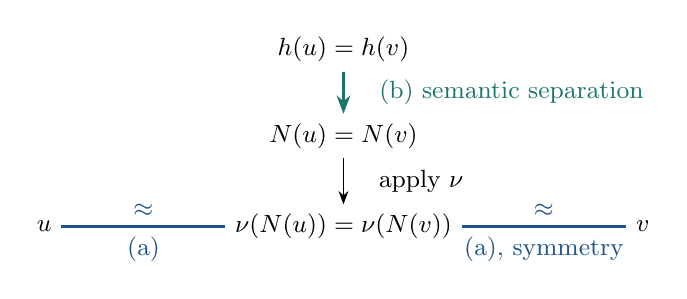
\begin{tikzpicture}[font=\small,>=Stealth]
\node (geo) at (0,2) {$h(u)=h(v)$};
\node (code) at (0,0.9) {$N(u)=N(v)$};
\draw[->,pathteal,thick] (geo) -- (code)
 node[midway,right] {\quad(b) semantic separation};
\node (common) at (0,-0.25) {$\nu(N(u))=\nu(N(v))$};
\draw[->] (code) -- (common) node[midway,right] {\quad apply $\nu$};
\node (u) at (-3.8,-0.25) {$u$};
\node (v) at (3.8,-0.25) {$v$};
\draw[pathblue,thick] (u) -- (common)
 node[midway,above] {$\approx$} node[midway,below] {(a)};
\draw[pathblue,thick] (common) -- (v)
 node[midway,above] {$\approx$} node[midway,below] {(a), symmetry};
\end{tikzpicture}
\caption{A normal-form certificate proves completeness by two different
means: syntactic normalization (a) connects each trace to its chosen normal
representative; semantic separation (b) forces the two codes to agree.
The bottom row is then scoped transitivity, yielding $u\approx v$.
The arrows are logical steps and assume nothing about continuity of $N$ or
$\nu$.}
\label{fig:normal-form}
\end{figure}


\begin{corollary}[fiberwise normal-form completeness]\label{cor:fiberwise-normal-form}
For fixed endpoints $a,b\in X$, the same definitions and proof apply to
$T(a,b)\subseteq T$.
In particular, a normal-form certificate on $T(a,a)$ proves geometric
completeness of the based-loop comparison on that fiber.
\end{corollary}

\begin{proof}
All endpoint maps and the scoped relation preserve fixed endpoint fibers, so
the two normal-form clauses and the proof of the criterion restrict to
$T(a,b)$ without change.
\end{proof}

\section{The universal presentation}
\label{sec:universal}

For every topological space $X$, take the primitive step space to be the
continuous interval path space $X^I$.  Its endpoint maps are evaluation at
$0$ and $1$.  Declare two parallel traces to be named generators exactly when
their realized paths are endpoint-fixed homotopic.
Thus every continuous path $\gamma$ is itself available as a one-letter
primitive trace.  If two realizations are endpoint-fixed homotopic, that
homotopy is literally one of the declared universal rules.  The universal
presentation is therefore complete in one step: the ambient homotopy relation
is built into the presentation instead of being derived from a normalizer.

The two lemmas below treat both representative topologies explicitly.
Without a superscript, $T_{\mathcal U_X}$ and $G_{\mathcal U_X}$ refer to the
observable choice.

\begin{lemma}[coherent-path quotient identification]
\label{lem:coherent-path-quotient-identification}
For the universal presentation, the projection
\[
  \pi:T_{\mathcal U_X}\longrightarrow X^I,
  \qquad \pi(p,\gamma)=\gamma,
\]
is a continuous quotient map.  Consequently, the quotient of
$T_{\mathcal U_X}$ by endpoint-fixed homotopy of the chosen representative is
canonically homeomorphic to the usual quotient-topologized path-class space
\[
  \Pi_1^q(X)=X^I/{\simeq_{\partial I}},
\]
with the endpoint maps retained.
\end{lemma}

\begin{proof}
For $T_{\mathrm{obs}}$, continuity of $\pi$ is immediate from the fifth
coordinate of $\kappa_{\mathrm{obs}}$.  For $T_{\mathrm{tr}}$, it is the
restriction of the second projection
$\mathsf{Tr}_{\mathcal P}\times X^I\to X^I$.  Every $\gamma\in X^I$ has the
coherent representative
\[
  \sigma(\gamma)=(\langle\gamma\rangle,\gamma),
\]
where $\langle\gamma\rangle$ is the one-letter universal trace and the
coherence is the constant endpoint-fixed homotopy.  The map $\sigma$ is
continuous on the one-letter coproduct component for $T_{\mathrm{tr}}$; it is
also continuous for $T_{\mathrm{obs}}$ because its observable code is built
continuously from $\gamma$.  Since $\pi\sigma=\mathrm{id}$, if
$\pi^{-1}(U)$ is open then
$U=\sigma^{-1}(\pi^{-1}(U))$ is open.  Thus $\pi$ is quotient.  The general quotient-factorization
lemma applied to the homotopy relation now induces mutually inverse
continuous maps between the two displayed quotient spaces.
\end{proof}

\begin{lemma}[fiberwise coherent-path quotient]
\label{lem:fiberwise-coherent-path-quotient}
Fix $a,b\in X$, and let
\[
  X^I(a,b)=\{\gamma\in X^I:\gamma(0)=a,\ \gamma(1)=b\}
\]
carry its subspace topology.  For $*=\mathrm{tr},\mathrm{obs}$, define the
coherent carrier with these fixed endpoints
\[
  T_{\mathcal U_X}^{*}(a,b)=
  \{(p,\gamma)\in T_{\mathcal U_X}^{*}:s(p)=a,\ t(p)=b\}
\]
with its own subspace topology, and define
$G_{\mathcal U_X}^{*}(a,b)$ to be its quotient by scoped equivalence, with
the quotient topology.  The restricted projection
\[
  \pi_{a,b}^{*}:T_{\mathcal U_X}^{*}(a,b)\longrightarrow X^I(a,b)
\]
is quotient.  Hence $G_{\mathcal U_X}^{*}(a,b)$ is canonically homeomorphic
to the endpoint-fixed homotopy quotient of $X^I(a,b)$.
\end{lemma}

\begin{proof}
The projection is continuous for either representative topology.  Its
one-letter section
\[
  \sigma_{a,b}(\gamma)=(\langle\gamma\rangle,\gamma)
\]
lands in the fixed endpoint fiber and is continuous by the same coordinate
argument as in Lemma~\ref{lem:coherent-path-quotient-identification}.
If $(\pi_{a,b}^{*})^{-1}(U)$ is open, then
$U=\sigma_{a,b}^{-1}((\pi_{a,b}^{*})^{-1}(U))$ is open.  Thus the restricted
projection is quotient without appealing to a restriction theorem for the
global projection.  In the universal presentation, scoped equivalence on this
fiber is exactly endpoint-fixed homotopy, so quotient factorization gives the
claimed homeomorphism.
\end{proof}

Two ingredients are needed for the universal identification
(Figure~\ref{fig:universal-section}).  The continuous
one-letter section makes representative projection a quotient map.  The
universal rewrite rules then identify scoped equivalence with endpoint-fixed
homotopy.  A section alone would not identify an arbitrary scoped quotient
with the ambient path-class space; the two relations must agree as well.

\begin{theorem}[universal completion]\label{thm:universal-completion}
For the universal presentation $\mathcal U_X$, scoped rewrite equality of
parallel traces is equivalent to endpoint-fixed homotopy of their realizations.
Consequently,
\[
  G_{\mathcal U_X}\cong \Pi_1^q(X)
\]
as abstract groupoids, and the comparison is a homeomorphism on arrow spaces.
\end{theorem}

\begin{proof}
Soundness is the general soundness theorem.  Conversely, an endpoint-fixed
homotopy is itself one of the named universal generators, so it is a scoped
rewrite in one step.  The equivalence of quotient relations follows after
including endpoint equality.  The coherent-path quotient identification lemma
supplies the missing topological identification with $\Pi_1^q(X)$, and the
geometric completeness theorem then gives the homeomorphism and groupoid
isomorphism.
\end{proof}

\begin{corollary}[collapse of the two universal topologies]
\label{cor:universal-topology-collapse}
For the universal presentation, the comparison map from
Proposition~\ref{prop:trace-sensitive-refinement}
\[
  J_{\mathcal U_X}:G_{\mathcal U_X}^{\mathrm{tr}}
    \longrightarrow G_{\mathcal U_X}^{\mathrm{obs}}
\]
is a homeomorphism.  More precisely, both spaces are canonically
homeomorphic to $\Pi_1^q(X)$, and these homeomorphisms identify
$J_{\mathcal U_X}$ with the identity on path classes.
\end{corollary}

\begin{proof}
The coherent-path quotient identification lemma applies to both representative
topologies and identifies each universal scoped quotient with
$\Pi_1^q(X)$.  The quotient maps are induced by the same representative
realization $\gamma$, so the two identifications commute with the identity on
path classes.  Hence the comparison map in
Proposition~\ref{prop:trace-sensitive-refinement}
is the composite of one homeomorphism with the inverse of the other, and is
therefore a homeomorphism.
\end{proof}

\begin{figure}[htbp]
\centering
\begin{tikzcd}[column sep=5em,row sep=4em,
 every label/.append style={font=\normalsize},
 every cell/.append style={font=\large}]
 X^I \arrow[r,shift left=1ex,"\sigma"] \arrow[d,"q_I"']
 & T_{\mathcal U_X}^{*} \arrow[l,shift left=1ex,"\pi"] \arrow[d,"q_*"] \\
 \Pi_1^q(X) \arrow[r,shift left=1ex,"\overline\sigma"]
 & G_{\mathcal U_X}^{*} \arrow[l,shift left=1ex,"\overline\pi"]
\end{tikzcd}

\smallskip
\(\displaystyle
 \pi\sigma=\mathrm{id}_{X^I},\qquad
 G_{\mathcal U_X}^{\mathrm{tr}}\cong\Pi_1^q(X)
 \cong G_{\mathcal U_X}^{\mathrm{obs}}.
\)
\caption{The universal one-letter section supplies the topology, and the
universal rules supply the equivalence relation.  Here
$*\in\{\mathrm{tr},\mathrm{obs}\}$ and
$\sigma(\gamma)=(\langle\gamma\rangle,\gamma)$; $q_I$ is the homotopy
quotient map.  The lower maps are induced by $\sigma$ and $\pi$.
The upper maps are continuous, with $\pi\sigma=\mathrm{id}$, so $\pi$ is
quotient.  Agreement of scoped and homotopy relations makes the lower maps
mutually inverse homeomorphisms.  Under these identifications, $J_{\mathcal U_X}$
is the identity on path classes.}
\label{fig:universal-section}
\end{figure}


\begin{proposition}[the universal path projection]
\label{prop:universal-path-projection}
Let $q_I^{\mathcal U}:X^I\to G_{\mathcal U_X}^{\mathrm{obs}}$ send a path to
the class of its one-letter coherent representative.  This map is quotient.
If $q_I^{\mathcal U}$ is open, the universal presentation has
product-quotient compatibility, and multiplication is continuous on the
ordinary pullback of its arrow space.
\end{proposition}

\begin{proof}
The geometric-path projection $r:T_{\mathcal U_X}^{\mathrm{obs}}\to X^I$
is continuous and has the continuous one-letter section $\sigma$.
Every coherent representative has the same scoped class as the one-letter
representative of its geometric path.  Thus
$q_T=q_I^{\mathcal U}\circ r$ and
$q_I^{\mathcal U}=q_T\circ\sigma$.  The first identity and the quotient
property of $q_T$ make $q_I^{\mathcal U}$ quotient.

On composable pairs, $r\times r$ again has a continuous section, so its
restriction to the endpoint pullbacks is quotient.  If
$q_I^{\mathcal U}$ is open, its square remains an open quotient after
restriction to the full inverse image of composable arrow pairs.
The composite is the ordinary pair map for $\mathcal U_X$.
The ordinary/final comparison theorem now gives product-quotient
compatibility and continuity of multiplication.
\end{proof}

\begin{theorem}[a positive geometric class]
\label{thm:universal-open-groupoid}
Let $X$ be locally path-connected and semilocally simply connected.  The
universal observable presentation $\mathcal U_X$ has product-quotient
compatibility.  Its scoped quotient is therefore a topological groupoid for
the ordinary pullback topology.  For every $x\in X$, the based arrow fiber
$G_{\mathcal U_X}(x,x)$ with the subspace topology from the global arrow
space is discrete, and its multiplication is continuous on the ordinary
product.
\end{theorem}

\begin{proof}
Holkar, Hossain, and Kulkarni prove that the path-class projection
$q_I:X^I\to\Pi_1^q(X)$ is open under these hypotheses
\cite[Corollary~3.7]{HolkarHossainKulkarni24}; their
Theorem~3.9 also identifies the resulting ordinary topological groupoid.
The arrow-space homeomorphism of
Theorem~\ref{thm:universal-completion} identifies $q_I$ with
$q_I^{\mathcal U}$.  Proposition~\ref{prop:universal-path-projection}
therefore gives product-quotient compatibility and continuous ordinary
multiplication.

The based arrow fiber is carried by that homeomorphism to the subspace of
$\Pi_1^q(X)$ with both endpoints $x$.  This subspace has the usual
based-loop quotient topology: the based-loop space is the full inverse
image of the fiber under the open map $q_I$, so the restricted map is still
open and quotient.  The one-letter section gives the same quotient topology
from the coherent based fiber.  Local path-connectedness and semilocal
simple connectivity make the quotient fundamental group discrete
\cite[Corollary~3.10(iii)]{HolkarHossainKulkarni24}.  Its product is
therefore discrete, and multiplication is continuous.
\end{proof}

The Hawaiian earring in Proposition~\ref{prop:hawaiian-earring} is locally
path-connected and fails the semilocal hypothesis at its common base point.
The two cases show how the ordinary-pullback obstruction behaves in geometric
presentations.  The positive groupoid theorem above is an application of the
published compact-open quotient result; the presentation-level comparison is
the contribution here.

\section{Circle and torus presentations}
\label{sec:circle-torus}

These examples use traces whose endpoints are the chosen base point.
Throughout this section, $G_{\mathcal P}(a,a)$ means the quotient of the
coherent based-loop carrier $T(a,a)$ with its own quotient topology.
It is not assumed to have the subspace topology inherited from the global
arrow quotient.  We first reduce words by the scoped rules, then use
winding numbers to distinguish the resulting normal forms.

\subsection{The additive circle: a finite generator and its completion}

Let $\mathbb T=\mathbb R/\mathbb Z$ carry the quotient topology.  The minimal
presentation has one oriented primitive step $a$ at the base point $0$, with
realization
\[
  a(t)=[t]\in\mathbb T.
\]
The formal reversal supplies $a^{-1}$; no integer-indexed primitive step is
assumed.  A based trace is therefore a finite signed word in $a$ and
$a^{-1}$.  No additional cancellation generator is needed: the structural
inverse coherences in Definition~\ref{def:scoped-rewrite-equality} instantiate to
\(a;a^{-1}\RwEq1_0\) and \(a^{-1};a\RwEq1_0\), and are closed under the
scoped congruence.

For a signed word $w$, let $\operatorname{exp}(w)$ be the number of positive
letters minus the number of negative letters.  Let $c_n$ be the canonical
word consisting of $n$ copies of $a$ when $n\geq 0$ and $-n$ copies of
$a^{-1}$ when $n<0$.

\begin{lemma}[finite-generator reduction]
Every signed word $w$ has a finite scoped derivation
\[
  w\RwEq c_{\operatorname{exp}(w)}.
\]
If two canonical words have endpoint-fixed homotopic realizations, then their
exponents are equal.  In particular, scoped-equivalent canonical words have
equal exponents by soundness.
\end{lemma}

\begin{proof}
Scan the word from left to right while retaining a reduced signed word.  If
the next sign agrees with the last retained sign, append it.  If the signs
differ, delete the adjacent inverse pair using the corresponding structural
coherence inside the surrounding prefix and suffix, using concatenation
congruence.  Each deletion strictly decreases the word length, so the
procedure terminates.  A terminal reduced word has no adjacent sign change
and hence consists entirely of positive letters or entirely of negative
letters.  The integer $\operatorname{exp}$ is unchanged by every deletion,
so the terminal word is exactly $c_{\operatorname{exp}(w)}$.  The same
invariant is the endpoint of the lift to $\mathbb R$; therefore endpoint-fixed
homotopy of canonical words forces equality of their exponents.
\end{proof}

For example, the cancellation mechanism gives the concrete scoped reduction
\[
  a;a^{-1};a^{-1};a;a
  \;\RwEq\;a^{-1};a;a
  \;\RwEq\;a.
\]
The first step cancels the initial $a;a^{-1}$ pair and the second cancels the
remaining $a^{-1};a$ pair.

The reduction lemma is the normal-form certificate from
Section~\ref{sec:comparison}: the reduction derivation gives clause (a), and the lifted endpoint
gives clause (b).  Thus the
minimal circle presentation is geometrically complete on its based loop
fiber.

It is also useful to package the derived integer normal forms as a completed
presentation with a primitive step $\lambda_n$ for each $n\in\Z$,
\[
  \lambda_n(t)=[tn].
\]
Its named rules are the derived integer rules
\[
  (n;m)\RwEq(n+m),\qquad 1_0\RwEq 0,
  \qquad (n)^{-1}\RwEq(-n).
\]
This integer-indexed presentation packages normal forms already derived
from the single generator.  The proof of the finite-generator classification
does not use it.

Let $L$ be the endpoint-fixed homotopy quotient of the based circle loop space,
with its quotient topology.  The map sending a loop class to its winding
number and the map
sending $n$ to the standard loop class are inverse maps.
Under the completeness conclusion below, write
\[
  S_0:L\longrightarrow G_{\mathcal P}(0,0)
\]
for the inverse of the realization comparison on the based-loop fiber.

\begin{theorem}[circle winding classification]
\label{thm:circle-winding}
The finite-generator scoped presentation is geometrically complete on the
based loop fiber, and winding number is a group isomorphism and a
homeomorphism
\[
  L\cong\Z,
\]
where $\Z$ is discrete.
Moreover, the inverse realization comparison
\[
  S_0:L\xrightarrow{\ \cong\ }G_{\mathcal P}(0,0)
\]
is a homeomorphism.  In particular the scoped presentation is
nondegenerate: the images of the zero and one winding loops are distinct.
\end{theorem}

\begin{proof}
A based loop has a unique lift to $\mathbb R$ starting at $0$.
Its endpoint is an integer, and endpoint-fixed homotopy preserves that
integer.  Straight-line interpolation of the lift with $t\mapsto tn$
shows that every loop of winding $n$ is homotopic to $\lambda_n$.
The lift of a concatenation is the first lift followed by a translate of the
second, so winding is additive.  Thus winding identifies $L$ with $\mathbb Z$
as groups.

The preceding reduction lemma sends every trace to $c_n$, where $n$ is
its winding number, so the normal-form criterion gives geometric
completeness.  Explicitly, $S_0$ sends a loop class of winding $n$ to
$q(c_n,\lambda_n)$.  Every scoped class has this form by normalization,
and soundness prevents different windings from giving the same scoped
class.  Hence $S_0$ is inverse to realization.  In particular, the zero
and one winding classes are distinct.



It remains to prove continuity of $S_0$.  Give $\mathbb T$ its standard
quotient metric.  If two based loops $\gamma,\delta$ are uniformly less
than $1/2$ apart, their difference has a unique continuous representative
$d:I\to(-1/2,1/2)$, with $d(0)=d(1)=0$.
Then $\gamma(t)+[u\,d(t)]$ joins them relative to endpoints.
Compact-open and uniform topologies agree here since $I$ is compact and
$\mathbb T$ is metric.  Winding is therefore locally constant and descends
continuously from $L$ to discrete $\Z$.
Choosing $(c_n,\lambda_n)$ for each $n$ gives a continuous map from
discrete $\Z$ to the coherent carrier and then to its scoped quotient.
This constructs $S_0$ continuously; projection to the chosen loop
supplies its continuous inverse.  The argument needs no result about
restrictions of quotient maps.  What it shows to be discrete is the based
loop-class quotient; it says nothing about the loop space itself.
\end{proof}



\subsection{The torus and its two generators}

Let
\[
  \mathbb T^2=(\mathbb R/\mathbb Z)\times(\mathbb R/\mathbb Z)
\]
with base point $(0,0)$.  Use two finite oriented generators
\[
  a(t)=([t],[0]),
  \qquad b(t)=([0],[t]).
\]
The only named rule is the commuting square
\[
  a;b\RwEq b;a;
\]
inverse cancellations for $a$ and $b$ are structural, as for the circle.
The commuting square is sound: it is the projection modulo $\mathbb Z^2$ of
the evident square homotopy in $\mathbb R^2$.  The other signed commutations
are derived, rather than added as generators.  For example, with unit
insertions and structural cancellations displayed schematically,
\[
\begin{aligned}
a^{-1};b
  &\RwEq a^{-1};(b;a);a^{-1}
   \RwEq a^{-1};(a;b);a^{-1}
   \RwEq b;a^{-1},\\
a;b^{-1}
  &\RwEq b^{-1};(b;a);b^{-1}
   \RwEq b^{-1};(a;b);b^{-1}
   \RwEq b^{-1};a,\\
b^{-1};a^{-1}
  &\RwEq a^{-1};b^{-1}
\end{aligned}
\]
and symmetry gives the reversed orientations.  Thus closure under the
scoped congruence supplies all four signed commuting rules.

For a signed word $w$, let $m(w)$ and $n(w)$ be its signed counts of $a$ and
$b$.  Move every $b$-letter to the right using the commuting square and then
perform the two cancellation algorithms from the circle.  This is a finite
terminating derivation
\[
  w\RwEq a^{m(w)};b^{n(w)}.
\]
The pair $(m(w),n(w))$ is invariant under every scoped rule.
Each signed commutation strictly decreases the number of pairs in which a
$b^{\pm1}$-letter occurs to the left of an $a^{\pm1}$-letter.
For a short worked instance, sorting and cancellation give
\[
  b;a;b^{-1};a;b
  \;\RwEq\;a;b;b^{-1};a;b
    \;\RwEq\;a;a;b
  \;=\;a^2;b.
\]
The first step uses the commuting square and the second cancels $b;b^{-1}$;
the winding pair is $(2,1)$.

\begin{lemma}[simultaneous and sequential torus representatives]
\label{lem:torus-sequential}
Let
\[
  d_{m,n}(t)=([mt],[nt])
\]
be the simultaneous standard loop, and let $|a^m;b^n|$ be the equal-slot
realization of the sequential word.  Then
\[
  d_{m,n}\simeq_{\partial I}|a^m;b^n|.
\]
\end{lemma}

\begin{proof}
Choose lifts of both loops to paths in $\mathbb R^2$ beginning at $(0,0)$.
The lift of $d_{m,n}$ is $t\mapsto(mt,nt)$, while the lift of the sequential
equal-slot realization is piecewise linear.  Both lifts end at $(m,n)$.
The straight-line interpolation between these two lifted paths is therefore
fixed at both endpoints.  Composing it with the covering map
$\mathbb R^2\to\mathbb T^2$ gives the required endpoint-fixed homotopy.
\end{proof}

Let $L_{\mathbb T^2}$ be the endpoint-fixed homotopy quotient of the based
loop space of $\mathbb T^2$, with its quotient topology.  Under geometric
completeness, write
\[
  S_{\mathbb T^2}:L_{\mathbb T^2}\longrightarrow
  G_{\mathcal P}((0,0),(0,0))
\]
for the inverse of the realization comparison on the based-loop fiber.

\begin{theorem}[torus winding classification]
\label{thm:torus-winding}
For the torus $\mathbb T^2$, the coordinate winding pair is a group
isomorphism and a homeomorphism
\[
  L_{\mathbb T^2}\cong\Z\times\Z,
\]
where $\Z\times\Z$ is discrete.
The finite-generator scoped presentation is geometrically complete on the
based loop fiber.  Moreover, the inverse realization comparison
\[
  S_{\mathbb T^2}:L_{\mathbb T^2}\xrightarrow{\ \cong\ }
  G_{\mathcal P}((0,0),(0,0))
\]
is a homeomorphism.
\end{theorem}

\begin{proof}
The universal cover is the product map
\[
  \mathbb R^2\longrightarrow\mathbb T^2,
  \qquad (x,y)\longmapsto([x],[y]).
\]
The lift of a based loop has endpoint $(m,n)\in\mathbb Z^2$, and endpoint-fixed
homotopy preserves this pair.  Conversely, the two coordinate projections of
any based torus loop are circle loops; the circle lifting theorem gives
endpoint-fixed homotopies to the standard loops of windings $m$ and $n$.
Taking their product gives a homotopy to the simultaneous loop $d_{m,n}$;
Lemma~\ref{lem:torus-sequential} then gives a homotopy to the sequential
realization $|a^m;b^n|$.  Thus the coordinate winding pair classifies
geometric loops, and it is additive because each coordinate winding is.  The word reduction above gives the corresponding scoped
derivation, so the normal-form criterion proves geometric completeness.
Projection from coherent representatives to their chosen loops induces
the continuous realization comparison.  The local-constancy argument
constructs its inverse continuously: each coordinate
winding number is locally constant by the circle argument.  The winding pair thus
descends continuously to discrete $\Z^2$, and the map
$(m,n)\mapsto(a^m;b^n,d_{m,n})$ is continuous because its domain is discrete.
Lemma~\ref{lem:torus-sequential} ensures that each pair is coherent.
Composing these maps with the scoped quotient map gives $S_{\mathbb T^2}$.
As for the circle, only the based loop-class quotient is shown to be
discrete.
\end{proof}

Figure~\ref{fig:winding} illustrates the lifted paths used in both proofs.
\begin{figure}[htbp]
\centering
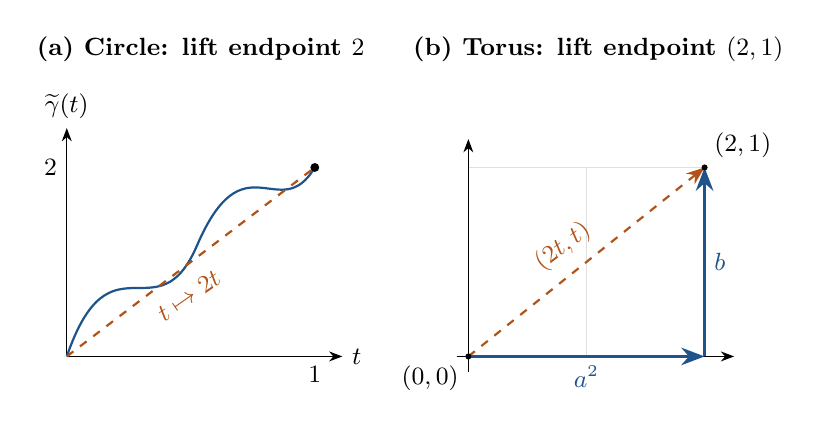
\begin{tikzpicture}[font=\small,>=Stealth]
\node[font=\small\bfseries] at (1.7,3.9) {(a) Circle: lift endpoint $2$};
\draw[->] (0,0) -- (3.5,0) node[right] {$t$};
\draw[->] (0,0) -- (0,2.9) node[above] {$\widetilde\gamma(t)$};
\draw[pathblue,thick] (0,0) .. controls (0.55,1.6) and (1.15,0.25) .. (1.65,1.4)
 .. controls (2.25,2.8) and (2.7,1.65) .. (3.15,2.4);
\draw[pathorange,thick,dashed] (0,0) -- (3.15,2.4);
\fill (3.15,2.4) circle (1.6pt);
\node[left] at (0,2.4) {$2$};
\node[below] at (3.15,0) {$1$};
\node[pathorange,rotate=35] at (1.55,0.77) {$t\mapsto 2t$};
\node[font=\small\bfseries] at (6.75,3.9) {(b) Torus: lift endpoint $(2,1)$};
\begin{scope}[xshift=5.1cm,x=1.5cm,y=2.4cm]
\draw[step=1,gray!25,very thin] (0,0) grid (2,1);
\draw[->] (-0.1,0) -- (2.25,0);
\draw[->] (0,-0.08) -- (0,1.15);
\draw[pathblue,very thick,->] (0,0) -- (2,0);
\draw[pathblue,very thick,->] (2,0) -- (2,1);
\draw[pathorange,thick,dashed,->] (0,0) -- (2,1);
\fill (0,0) circle(1.1pt) node[below left] {$(0,0)$};
\fill (2,1) circle(1.1pt) node[above right] {$(2,1)$};
\node[pathblue,below] at (1,0) {$a^2$};
\node[pathblue,right] at (2,0.5) {$b$};
\node[pathorange,rotate=37] at (0.8,0.58) {$(2t,t)$};
\end{scope}
\end{tikzpicture}
\caption{Winding separates normal forms because lifts remember endpoints.
Left: a lift beginning at $0$ and ending at $2$ is straightened to $2t$.
Right: the sequential word $a^2;b$ and the simultaneous loop have lifts
with common endpoints $(0,0)$ and $(2,1)$; straight-line interpolation in
$\mathbb R^2$ gives a homotopy after projection to the torus.
Both plots are drawn in the covering spaces $\mathbb R$ and $\mathbb R^2$.}
\label{fig:winding}
\end{figure}


\subsection{Products of complete based presentations}

The torus sorting argument extends to a product without requiring normal
forms for either factor.  Let $\mathcal P$ be a sound scoped presentation
on $X$ with primitive steps $E$, and let $\mathcal Q$ be one on $Y$ with
primitive steps $F$.  A product trace has horizontal letters $(e,y')$ and
vertical letters $(x',f)$, where $e\in E$, $f\in F$, $x'\in X$, and
$y'\in Y$.  Their realizations hold the other coordinate fixed.  Lift each
named rule of $\mathcal P$ at every $y'$, and each rule of $\mathcal Q$ at
every $x'$.  Add interchange around every primitive rectangle:
\[
 (e,y_0);(x_1,f)\ \simeq_{\mathcal P\boxtimes\mathcal Q}\
 (x_0,f);(e,y_1),
 \quad e:x_0\to x_1,\quad f:y_0\to y_1.
\]
We also name the corresponding rule for arbitrary factor traces $p:x_0\to x_1$
and $q:y_0\to y_1$:
\[
 H_{y_0}(p);V_{x_1}(q)\ \simeq_{\mathcal P\boxtimes\mathcal Q}\
 V_{x_0}(q);H_{y_1}(p).
\]
Here $H_y$ and $V_x$ lift entire traces while holding the other coordinate
fixed.  Write $\mathcal P\boxtimes\mathcal Q$ for this presentation.
The rules are sound: the two paths are the two edge routes from $(x_0,y_0)$
to $(x_1,y_1)$ in the square
$(u,v)\mapsto(\rho(e)(u),\rho(f)(v))$.  The routes are homotopic relative
to their endpoints inside the square.  The same construction with the
realizations of $p$ and $q$ proves soundness for the trace rule.  Naming it
makes the sorting argument direct; we do not claim here that all such rules
have been derived from the primitive squares in the formalization.

\begin{theorem}[product closure of based completeness]
\label{thm:product-completeness}
Suppose $\mathcal P$ is geometrically complete on the based-loop fiber at
$x\in X$ and $\mathcal Q$ is geometrically complete on the based-loop
fiber at $y\in Y$.  Then $\mathcal P\boxtimes\mathcal Q$ is geometrically
complete on the based-loop fiber at $(x,y)$.
\end{theorem}

\begin{proof}
Induct on a product trace.  Reflection and single letters are already
sorted after inserting a unit trace.  For a concatenation, first sort both
parts, then use the trace interchange rule to move the first part's
vertical projection past the second part's horizontal projection.
For an inverse, reverse the sorted trace and use interchange once more.
Thus every trace rewrites to its horizontal projection followed by its
vertical projection.  Since the
entire trace starts and ends at $(x,y)$, the horizontal projection is a loop at
$x$, lifted at $y$, and the vertical word is a loop at $y$, lifted at $x$.

Take two coherent product loops whose geometric representatives are
endpoint-fixed homotopic.  Soundness and coherence let us replace each by
its sorted realization.  Projecting the resulting homotopy to $X$ gives a
homotopy between the two horizontal realizations: every vertical letter
projects to a constant segment, which can be removed by an endpoint-fixed
reparametrization homotopy.  Projection to $Y$ gives the corresponding
homotopy between vertical realizations.  Completeness of $\mathcal P$ and
$\mathcal Q$ supplies scoped derivations between the respective factor
words.  Lift the first derivation at $y$ and the second at $x$, then compose
them with the two sorting derivations.  This is a scoped derivation between
the original product words, as required.
\end{proof}

Iterating the theorem from the finite oriented circle presentation gives
completeness of the corresponding product presentation of every
$n$-torus on its based-loop fiber.  It has finitely many primitive steps,
though its named trace-interchange rules form a schema.  For $n=2$, it
recovers the completeness conclusion of Theorem~\ref{thm:torus-winding}.
The Lean development checks the product presentation, its sorting derivation,
and the based trace-completeness theorem under exactly these rules.

\section{Relation to logic and rewriting}
\label{sec:logic}

In logical terms, a scoped derivation proves an equality in the presented
groupoid $G_{\mathcal P}$, and soundness sends that equality to an equality of
geometric homotopy classes.  Normal forms can prove the converse for a
particular presentation.  In the universal presentation the converse holds by
definition, since every endpoint-fixed homotopy is a named rewrite.

The semantic factorization theorem (Theorem~\ref{thm:semantic-factorization})
is the logical universal property of the construction.  At this level, a
scoped derivation is a finite proof object built from named rules and
structural constructors; soundness is an induction principle on that
derivation.  Completeness is a separate theorem: whenever two represented paths are
homotopic, their traces are related by the allowed rewrites.  It is about
equality of represented homotopy classes; individual homotopy witnesses are
not represented.

The construction is compatible with the standard algebra of rewriting
\cite{ChurchRosser36,Newman42,KnuthBendix70,Squier87,GuiraudMalbos09}:
congruence, symmetry, and transitivity are already part of scoped equality.
Additional named rules require homotopy witnesses, as in the definition of a
presentation.  Termination and confluence are not assumptions of the
topological construction.  They may help establish a normalizer, but the
normal-form criterion still requires both a scoped normalization derivation
and a proof that geometrically equivalent inputs have the same code.
The finite-generator circle and torus reductions discharge those checks
explicitly.

The quotient keeps trace classes and forgets the derivations between them,
in the same way that coherence asks for a homotopy to exist and forgets which
one.  Computational data are used before quotienting; after quotienting,
arrows are compared by ordinary equality.  The construction does not produce
a proof-relevant identity type or a higher groupoid of homotopy witnesses.

\section{What the Lean developments check}
\label{sec:formalization}

Two Lean developments accompany the paper.  The parent artifact
(Section~\ref{sec:parent-artifact}) uses Lean 4.24.0 and Mathlib 4.24.0 and covers the constructions
listed in Table~\ref{tab:declarations}.  A smaller extraction, built with
Lean~4.32.0, contains one bundled statement registered in Palomar
(Section~\ref{sec:palomar}).  The statements and proofs in this paper can be read without
either implementation, and in both cases the checks cover the named
declarations and nothing else.

\subsection{The parent artifact}
\label{sec:parent-artifact}

\paragraph{Traces, soundness, and quotient operations.}
The implementation represents traces by the parenthesized inductive type
\LeanName{GeometricTrace}, where Section~\ref{sec:traces} uses flat signed words.  The
declarations \LeanName{WeightedSlotReparam},
\LeanName{balancedSlotReparam}, and
\LeanName{weightedConcatenationInvariant} relate the two parametrizations,
including the null-homotopy assumptions needed when a factor has zero weight.
The scoped-rewrite modules check soundness and the quotient operations.  The
comparison with Mathlib's fundamental groupoid identifies the represented
homotopy classes, checks preservation of identities, inverses, and
composition, and proves that the induced map on final composable-pair domains
is continuous.

\paragraph{Representative topologies.}
The module \LeanName{TraceSensitiveTopologicalCompPath} flattens internal
traces to signed words.  It checks continuity of the full-word realization,
of the map to observable coordinates, and of the identity, reversal, and
weighted composition operations.  The earlier quotient modules still use the
observable topology by default.

The module \LeanName{TraceSensitiveSeparation} checks the two-label
separation mechanism on a finite code space: the one-letter trace codes
differ, their observable codes agree, and the identity from the discrete
trace topology to the indiscrete observable topology is continuous while its
inverse is not. It also checks that the two circle labels realize the same
nonconstant loop, proves the signed-count invariant for every structural
scoped rewrite, and separates their scoped quotient classes. Their full
observable codes agree. Signed count descends continuously to the
trace-sensitive quotient; the comparison to the observable quotient is
continuous, but its inverse is not. Thus the topological separation in
Example~\ref{ex:quotient-topology-separation} is checked in Lean. The module
\LeanName{TraceSensitiveUniversalCollapse} checks the continuous one-letter
section and the homeomorphism between the two universal quotient topologies.

\paragraph{Circle and torus examples.}
The module \LeanName{FiniteCircleTorusPresentation} uses one circle generator
and two torus generators.  It checks integer and integer-pair codes for
traces, completion certificates, and soundness of the torus commuting square.
The cancellation and sorting proofs of Section~\ref{sec:circle-torus} are still needed: they
establish normalization in the minimal scoped presentations, whereas the
completion certificates package normal forms through a specified relation.
The separate torus development in
\LeanName{ComputationalPaths/Path/Topology/TopologicalTorusScoped.lean}
includes the comparison between simultaneous and sequential loop
representatives.

\paragraph{Hawaiian-earring transfer.}
The dedicated module checks that an externally supplied failure of the
product-quotient property yields failure of ordinary-pair compatibility, and
it transfers discontinuity of multiplication along the comparison
homeomorphism.  Fabel's results enter as assumptions; the Lean development
does not reprove them.

\paragraph{Build and archive.}
The root import file is \LeanName{ComputationalPaths.lean}, and
Table~\ref{tab:declarations} in Appendix~\ref{app:declarations} lists the
principal declarations.  The core artifact, version
\texttt{0.6.1+lean-only-v3}, is archived on Zenodo under the version DOI
\href{https://doi.org/10.5281/zenodo.21938980}
{\nolinkurl{doi:10.5281/zenodo.21938980}}; its concept DOI is
\href{https://doi.org/10.5281/zenodo.21817207}
{\nolinkurl{doi:10.5281/zenodo.21817207}} \cite{RamosEtAl2026TopologyArtifact}.
The source, including the finite-generator module, the torus
simultaneous/sequential bridge, and the trace-sensitive topology module, is
also in the
\href{https://github.com/Arthur742Ramos/ComputationalPathsLean}{GitHub repository}.
Build the project with \texttt{lake build}; the artifact README lists commands
for building individual modules separately.

The checked modules contain no unfinished proofs and no custom axiom
declarations.  Declaration-level axiom inspection reports only Lean's standard
logical and quotient principles: propositional extensionality, classical
choice, and quotient soundness.  The development complements earlier work on
computational paths and the Lean theorem prover
\cite{deMoura2021,RamosEtAl2025LeanPreprint,RamosEtAl2025OmegaPreprint}.

\subsection{The registered result}
\label{sec:palomar}
The extraction
\href{https://github.com/Arthur742Ramos/TopologicalComputationalPaths}
{\emph{TopologicalComputationalPaths}} has a registered Palomar result,
\href{https://palomar-registry.org/entry?id=PALOMAR-2026-08-29-000005&version=1}
{\texttt{PALOMAR-2026-08-29-000005}}, version~1,
published on 29~August~2026 \cite{PalomarScoped2026}.
It selects the single bundled declaration
\LeanName{TopologicalComputationalPaths.main_result} at the immutable commit
\[
 \texttt{8254c40d0de03ff469c7c9c05087b8bc154e9a87},
\]
built with Lean~4.32.0 and its checked-in dependency manifest.  The selected
statement is an \LeanName{OrdinaryTopologyComparisonCertificate}, and
Table~\ref{tab:palomar-scope} summarizes what it covers.

The certificate has three parts.  The first gives the continuous bijection
between final and ordinary pair spaces, the equivalent criteria for their
topologies to agree, the compact-Hausdorff and discrete sufficient
conditions, the consequence for ordinary composition, and the obstruction
obtained from discontinuity.  (The discrete field assumes that both
$G_{\mathcal P}$ and its final domain are discrete; by
Corollary~\ref{cor:discrete} the first assumption implies the second.)  The
second part classifies based-loop homotopy classes of the circle and torus by
integers and integer pairs.  It checks the invariant, the standard
representatives, the identity value, additivity under concatenation, and that
the classification maps are mutually inverse.  The homeomorphism statements
of Theorems~\ref{thm:circle-winding} and~\ref{thm:torus-winding} are not part
of it.  The third part transfers the Hawaiian-earring obstruction under the
hypotheses described below.

\begin{table}[htbp]
\centering\small
\begin{tabular}{>{\raggedright\arraybackslash}p{0.27\linewidth}
                >{\raggedright\arraybackslash}p{0.65\linewidth}}
\toprule
Part of the paper & Scope of the registered certificate\\
\midrule
Final/ordinary comparison &
Canonical continuous bijection; exact quotient/homeomorphism/topology
criteria; sufficient conditions and ordinary-composition consequence.\\
Circle and torus &
Additive classifications of the actual loop quotients, with explicit
standard representatives and inverse laws.\\
Hawaiian earring &
Concrete observable based fiber and quotient comparison; obstruction
transfer conditional on \LeanName{FabelHawaiianEarringFacts}.\\
Broader exposition &
Not certified by this selection: the trace-sensitive refinement, the
minimal finite-generator rewrite algorithms, the homeomorphism statements
for the circle and torus, the explanatory homotopies and figures, and the
manuscript as a whole.\\
\bottomrule
\end{tabular}
\caption{What the Palomar registration covers.  Supporting code and
mathematical exposition are listed apart from the selected conclusions.}
\label{tab:palomar-scope}
\end{table}

The Hawaiian-earring field needs a caveat.  In the registered statement, the
topology \LeanName{hawaiianObservableOpenFiberTopology} is induced by the
geometric projection alone, and its one-letter section identifies its
quotient with the standard loop quotient.  This topology was defined for the
registered based-fiber result; identifying it with the topologies of
Section~\ref{sec:traces} would need a proof.  The field \LeanName{hawaiian_based_fiber}
assumes \LeanName{FabelHawaiianEarringFacts}, so the failure of the
product-quotient property and the discontinuity of multiplication are
hypotheses there, and the extraction does not reprove them.  In the
mathematical account, Proposition~\ref{prop:hawaiian-earring} takes them
from Fabel's published result \cite{Fabel11}.

The current working source after that immutable version equips the Hawaiian
observable based carrier with the topology induced by its full observable
code.  The revised one-letter section and geometric projection are
continuous, and the based quotient remains homeomorphic to the usual loop
quotient.  It also weakens the discrete sufficient condition in the selected
certificate to discreteness of the arrow space alone, and checks continuity
of both projections from the final composable domain.  The present Lean
source also checks the general open-arrow criterion and
Proposition~\ref{prop:universal-path-projection}: the path-class projection
is quotient, and its openness implies ordinary multiplication for the
universal presentation.  The published openness theorem used in
Theorem~\ref{thm:universal-open-groupoid} has not been formalized here.

On fixed endpoint quotients, Lean now identifies the universal based fiber
with the ordinary based-loop quotient.  It proves discreteness, a quotient
pair map, and continuous ordinary multiplication under the semilocal
hypothesis. It also identifies based paths with the endpoint-defined
subspace of the compact-open path space and checks that an open global
projection restricts to an open quotient onto the based-arrow subspace.
Under this open-map hypothesis, Lean identifies that subspace fiber with
the ordinary based-loop quotient and proves it discrete under local
path-connectedness and semilocal simple connectivity. The open-map
hypothesis itself is supplied by the cited theorem, not by a Lean proof.
The integer-indexed scoped circle presentation has a checked normal form;
its fixed endpoint quotient is homeomorphic to $\mathbb Z$, and a continuous
winding-based trace choice identifies its trace-sensitive and observable
quotient topologies.  This integer-indexed certificate is distinct from the
finite-generator circle presentation in Section~\ref{sec:circle-torus}.
The current source also checks the general trace-section criterion, the
universal trace collapse, a finite separation model, and the realized
fundamental-groupoid arrow comparison.  For products it defines the
horizontal and vertical continuous step system, checks geometric soundness
of primitive and trace interchange, and proves sorting and based trace
completeness for the presentation in Theorem~\ref{thm:product-completeness}.
For the finite-generator circle and torus, it also checks continuous
winding-based choices of signed traces and the consequent based quotient
comparison under an explicit completeness hypothesis.  The completeness
proofs for those exact finite scoped presentations remain manuscript
arguments.
None of these working-source additions has been registered as a new Palomar
version.

To reproduce the selected result, check out the pinned commit and run
\texttt{lake build}.  The selection file \LeanName{comparator.json} pairs
\LeanName{Challenge.lean} with \LeanName{Solution.lean}.  The theorem
placeholder in \LeanName{Challenge.lean} states what is checked against the
proof in \LeanName{Solution.lean}, so it does not count as an unfinished
proof.  Later follow-up and preimage-solver development is outside this
registered snapshot.  Registration gives a versioned verification record for
the selected formal statement and nothing more.  It does not cover the prose
or the illustrations, and it implies neither journal acceptance nor an
endorsement of novelty.
\FloatBarrier

\section{Conclusion}
\label{sec:conclusion}

Two questions come up when computational paths are interpreted
geometrically, and this paper keeps them apart.  The first is algebraic:
which traces should count as equal?  A scoped presentation answers with its
declared rewrites and the groupoid laws.  Soundness guarantees that equal
traces realize homotopic paths, and the converse needs a completeness proof,
which the normal-form criterion supplies for the based-loop circle and torus
presentations.  The product theorem extends based completeness from two
presentations to their product, yielding finite-generator presentations for
all finite tori.

The second question is topological: on which space of composable classes is
multiplication continuous?  The quotient of composable representatives always
works.  Its topology need not agree with the ordinary subspace topology on
pairs of quotient arrows, and product-quotient compatibility is exactly the
condition under which the two agree.  An open arrow quotient guarantees this
compatibility.  Applied to the universal presentation, the published
open-map theorem for locally path-connected, semilocally simply connected
spaces yields an ordinary topological groupoid and discrete based fibers.
The Hawaiian earring shows that this conclusion does not extend to every
locally path-connected space.

In the universal presentation every path is a primitive step and every
endpoint-fixed homotopy is a rewrite, so its scoped quotient is the usual
fundamental groupoid with the quotient topology on arrows.  For a complete
presentation, a continuous choice of trace for each represented path also
identifies the trace-sensitive and observable quotient topologies.  This
applies to the universal presentation and the based-loop circle and torus
examples.  Section~\ref{sec:formalization} distinguishes the Lean checks
from the mathematical arguments and the immutable registered result.

\section*{Funding}
No external funding was received for this work.

\section*{Acknowledgements}
AI-assisted tools were used during manuscript preparation for editorial
support and assistance with software, documentation, and figure preparation.
The geometric exposition and figures were developed from Tiago M.~L.~de
Veras's suggestions on reversal, coherence, and homotopy obstructions.
The figures are mathematical schematics with explicitly stated maps and
boundary conditions.  They illustrate the arguments and are not offered as
evidence for the theorems.

\clearpage
\appendix
\section{Declaration index for the parent artifact}\label{app:declarations}
This index records the representative declarations discussed in Section~\ref{sec:parent-artifact}.
It describes the parent Lean artifact, not the independently registered
Palomar selection of Section~\ref{sec:palomar}.  Fully qualified names are retained for
source lookup.
\begingroup
\small
\renewcommand{\arraystretch}{1.12}
\begin{longtable}{>{\raggedright\arraybackslash}p{0.23\linewidth}>{\raggedright\arraybackslash}p{0.69\linewidth}}
\caption{Representative declarations in the parent artifact, not the Palomar selection.}\label{tab:declarations}\\
\toprule
Mathematical layer & Representative checked declarations\\
\midrule
\endfirsthead
\multicolumn{2}{l}{\small\itshape Table \thetable\ continued}\\
\toprule
Mathematical layer & Representative checked declarations\\
\midrule
\endhead
\bottomrule
\endfoot
Scoped syntax and soundness &
\LeanName{ScopedGeometricRewritePresentation},
\LeanName{ScopedRwEq}, \LeanName{ScopedRwEq.sound}\\
Weighted realization &
\LeanName{WeightedSlotReparam}, \LeanName{balancedSlotReparam},
\LeanName{weightedConcatenationInvariant}\\
Trace-sensitive topology &
\LeanName{TraceSensitiveTopologicalCompPath.lean},
\LeanName{continuous_fullTraceRealization},
\LeanName{continuous_traceSensitive_to_observable},
\LeanName{traceSensitiveTopologyCertificate},
\LeanName{TraceSensitiveQuotient.continuous_quotientComparison},
\LeanName{TraceSensitiveQuotient.quotientComparisonHomeomorph_of_realization_section}\\
Finite topology separation &
\LeanName{TraceSensitiveSeparation.oneLetter_e_ne_f},
\LeanName{TraceSensitiveSeparation.observableCode_e_eq_f},
\LeanName{TraceSensitiveSeparation.not_continuous_observable_to_trace},
\LeanName{TraceSensitiveSeparation.certificate}\\
Quotient groupoid and topology &
\LeanName{ScopedComposableClass},
\LeanName{scopedCompositionOnStrong},
\LeanName{scopedFinalTopologicalGroupoidCertificate}\\
Ordinary/final comparison &
\LeanName{scopedProductCompatibility_iff_four_way},
\LeanName{scopedProductCompatibility_of_compact_final_t2}\\
Comparison and normal forms &
\LeanName{ComparisonFunctorCertificate},
\LeanName{comparisonHomeomorph_of_complete},
\LeanName{ScopedGeometricNormalFormCertificate}\\
Universal and obstruction cases &
\LeanName{universalHomeomorph},
\LeanName{ScopedGeometricRewrite.universalTraceSensitiveHomeomorph},
\LeanName{QuotientObstructionTransfer},
\LeanName{MultiplicationComparison}\\
Finite-generator presentation data &
\LeanName{FiniteCircleTorusPresentation.circleFinitePresentation},
\LeanName{FiniteCircleTorusPresentation.circleCompletionEquivInt},
\LeanName{FiniteCircleTorusPresentation.torusFinitePresentation},
\LeanName{FiniteCircleTorusPresentation.torusCompletionEquivIntProd},
\LeanName{FiniteCircleTorusPresentation.torusFiniteCommutingSquare}\\
Completed circle and topological torus &
\LeanName{circleBasedNormalFormCertificate},
\LeanName{TopologicalTorus.standardLoop_homotopic_sequentialLoop},
\LeanName{TopologicalTorus.equivIntProd},
\LeanName{TopologicalTorus.certificate}\\
\end{longtable}
\endgroup

\clearpage
\bibliographystyle{amsplain}
\begingroup
\small
\bibliography{../refs}
\endgroup

\end{document}
